\UseRawInputEncoding
\documentclass{article}

\usepackage[utf8]{inputenc}
\usepackage[french]{babel}
\usepackage{listings}
\usepackage{xcolor}
\usepackage{graphicx}
\usepackage{amsmath}
\usepackage{hyperref}
\usepackage{float}
\usepackage{xurl}
\usepackage{microtype}
\usepackage{enumitem}
\usepackage{parskip}
\usepackage{subcaption}
\usepackage{geometry}

\geometry{margin=2.3cm}

\definecolor{codegreen}{rgb}{0,0.6,0}
\definecolor{codegray}{rgb}{0.5,0.5,0.5}
\definecolor{codepurple}{rgb}{0.58,0,0.82}
\definecolor{backcolour}{rgb}{0.95,0.95,0.92}

\lstdefinestyle{mystyle}{
    backgroundcolor=\color{backcolour},
    commentstyle=\color{codegreen},
    keywordstyle=\color{magenta},
    numberstyle=\tiny\color{codegray},
    stringstyle=\color{codepurple},
    basicstyle=\ttfamily\footnotesize,
    breakatwhitespace=false,
    breaklines=true,
    captionpos=b,
    keepspaces=true,
    numbers=left,
    numbersep=5pt,
    showspaces=false,
    showstringspaces=false,
    showtabs=false,
    tabsize=2
}

\lstset{style=mystyle}

\title{
Rapport de TP -- Simulateur à événements discrets\\
\large Séance 2/3 : clients, file d’attente, serveurs, configuration et tests
}

\author{
Groupe 3 \\ \\
PINCAUD Steve, SAVIARD Matthieu et CHARONNET Henri
}

\date{\today}

\begin{document}

\maketitle

\begin{abstract}
Ce rapport présente le travail réalisé lors de la deuxième séance du TP consacré à la construction d’un simulateur à événements discrets. La première séance avait permis de mettre en place les briques fondamentales du simulateur : messages, événements, ordonnanceur, moteur principal et traces. Cette deuxième séance poursuit l’architecture orientée objet en introduisant les composants opérationnels du système simulé : les clients, la file d’attente, les serveurs, les distributions aléatoires et la configuration globale.

L’objectif de cette séance est de préparer la simulation d’un système de file d’attente de type M/M/1, M/M/1/K ou M/M/c/K. Pour cela, le simulateur doit être capable de créer des entités clientes, de représenter une file d’attente FIFO, de modéliser un ou plusieurs serveurs, de charger une configuration commune et de préparer la génération de temps aléatoires. Le rapport détaille les responsabilités de chaque classe, les liens entre interfaces et implémentations, la stratégie de test et l’intégration progressive dans le fichier \texttt{Engine.py}.
\end{abstract}

\tableofcontents
\newpage

\section{Introduction}

La simulation à événements discrets permet d’étudier le comportement temporel d’un système en ne considérant que les instants où un changement d’état se produit. Dans le contexte du TP, le système modélisé correspond à une chaîne de traitement simplifiée composée de clients, d’une passerelle, d’une file d’attente et de serveurs.

Lors de la séance 1, les fondations du simulateur ont été mises en place :
\begin{itemize}[leftmargin=*]
    \item la classe \texttt{MessageImpl}, qui représente les messages échangés ;
    \item la classe \texttt{EventImpl}, qui représente les événements datés ;
    \item l’énumération \texttt{EventType}, qui définit les types d’événements ;
    \item la classe \texttt{SchedulerImpl}, qui maintient la liste chronologique des événements ;
    \item le fichier \texttt{Engine.py}, qui prépare le moteur de simulation ;
    \item le système de journalisation.
\end{itemize}

La séance 2 étend cette architecture avec les composants qui représentent l’activité réelle du système :
\begin{itemize}[leftmargin=*]
    \item la classe \texttt{ClientImpl}, chargée de modéliser les générateurs de messages ;
    \item la classe \texttt{QueueImpl}, chargée de représenter la file d’attente ;
    \item la classe \texttt{ServerImpl}, chargée de représenter les serveurs de traitement ;
    \item la classe \texttt{ConfigImpl}, chargée de centraliser la configuration ;
    \item les classes \texttt{Distribution} et \texttt{Poisson}, utilisées pour la génération aléatoire ;
    \item les interfaces associées : \texttt{IClient}, \texttt{IQueue}, \texttt{IServer}, \texttt{IConfig}.
\end{itemize}

Cette séance ne correspond pas encore à l’assemblage complet du simulateur final. Elle constitue cependant une étape essentielle : les objets métier nécessaires à la simulation sont maintenant identifiés, structurés et reliés par des interfaces.

\section{Objectifs de la séance 2}

D’après le planning du TP, la séance 2 porte sur :
\begin{itemize}[leftmargin=*]
    \item le \texttt{Main} et les méthodes de test ;
    \item la classe \texttt{Client} ;
    \item la classe \texttt{Queue} ;
    \item la classe \texttt{Server}.
\end{itemize}

L’objectif est donc d’enrichir le squelette du simulateur avec les entités qui interviendront directement dans la dynamique d’une file d’attente.

\subsection{Objectifs fonctionnels}

Les objectifs fonctionnels de cette séance sont les suivants :
\begin{enumerate}[leftmargin=*]
    \item représenter un ou plusieurs clients capables de générer des messages ;
    \item représenter une file d’attente contenant les messages en attente de traitement ;
    \item représenter un ou plusieurs serveurs capables de traiter des messages ;
    \item préparer la génération de temps inter-arrivées et de temps de service ;
    \item intégrer ces composants dans le moteur principal ;
    \item mettre en place des tests séparés pour chaque classe.
\end{enumerate}

\subsection{Objectifs logiciels}

D’un point de vue logiciel, la séance 2 poursuit plusieurs objectifs de conception :
\begin{itemize}[leftmargin=*]
    \item conserver une architecture orientée objet ;
    \item maintenir la séparation entre interfaces et implémentations ;
    \item centraliser les paramètres dans une classe de configuration ;
    \item utiliser le logging de manière homogène ;
    \item préparer l’extension vers la passerelle et les métriques de la séance 3 ;
    \item rendre les composants testables indépendamment.
\end{itemize}

\section{Rappel du modèle simulé}

\subsection{Architecture générale}

Le système simulé peut être représenté par la chaîne suivante :

\begin{center}
\texttt{Client(s) ->  Queue -> Server(s)}
\end{center}

Les clients génèrent des messages. Ces messages sont ensuite reçus par la passerelle. Si un serveur est disponible, le message peut être traité immédiatement. Sinon, il est placé dans une file d’attente. Lorsque le traitement se termine, un événement de départ est généré.

\subsection{Événements manipulés}

Les événements de base restent ceux de la séance 1 :
\begin{itemize}[leftmargin=*]
    \item \texttt{SEND\_MSG} : émission d’un message par un client ;
    \item \texttt{RECV\_MSG} : réception du message par la passerelle ;
    \item \texttt{MSG\_DEPT} : fin de traitement du message par un serveur.
\end{itemize}

L’énumération \texttt{EventType} centralise ces types d’événements :

\begin{lstlisting}[language=Python, caption=EventType.py]
from enum import Enum

## EventType – SEND_MSG, RECV_MSG, MSG_DEPT

class EventType(Enum):
    SEND_MSG = 1
    RECV_MSG = 2
    MSG_DEPT = 3
\end{lstlisting}

L’utilisation d’une énumération permet de limiter les erreurs liées aux chaînes de caractères libres. Elle rend également le code plus lisible, car les types d’événements sont déclarés en un seul endroit.

\subsection{Variables importantes du modèle}

Pour préparer les simulations de la séance 3, plusieurs variables devront être suivies :
\begin{itemize}[leftmargin=*]
    \item le temps courant de simulation ;
    \item le nombre de messages générés ;
    \item le nombre de messages reçus ;
    \item le nombre de messages servis ;
    \item le nombre de messages présents dans la file ;
    \item l’état des serveurs ;
    \item le nombre de messages rejetés dans les modèles à capacité finie ;
    \item les temps de séjour des messages.
\end{itemize}

La séance 2 prépare ces variables en introduisant les classes qui vont les porter ou les manipuler.

\section{Organisation du projet}

\subsection{Arborescence logique}

L’organisation du projet suit la structure suivante :

\begin{verbatim}
rcp103/
|-- tp2.log
|-- net/
    |-- lecnam/
        |-- rcp103/
            |-- tp2/
                |-- Engine.py
                |-- ConfigImpl.py
                |-- ConfigImplTest.py
                |-- Distribution.py
                |-- Poisson.py
                |-- MessageImpl.py
                |-- MessageImplTest.py
                |-- EventImpl.py
                |-- EventImplTest.py
                |-- EventImplMockTest.py
                |-- EventType.py
                |-- SchedulerImpl.py
                |-- ClientImpl.py
                |-- ClientImplTest.py
                |-- QueueImpl.py
                |-- QueueImplTest.py
                |-- ServerImpl.py
                |-- ServerImplTest.py
                |-- GatewayImpl.py
                |-- IConfig.py
                |-- IMessage.py
                |-- IEvent.py
                |-- IScheduler.py
                |-- IClient.py
                |-- IQueue.py
                |-- IServer.py
                |-- IGateway.py
                |-- logging_config.cnf
\end{verbatim}

Cette organisation permet de regrouper chaque concept dans un fichier séparé. Les fichiers préfixés par \texttt{I} correspondent aux interfaces, tandis que les fichiers suffixés par \texttt{Impl} correspondent aux implémentations concrètes.

\subsection{Commandes d’exécution}

Les fichiers de test peuvent être exécutés depuis la racine du projet avec la variable \texttt{PYTHONPATH} :

\begin{lstlisting}[language=bash, caption=Exécution des tests sous Linux ou WSL]
PYTHONPATH=. python3 net/lecnam/rcp103/tp2/ConfigImplTest.py
PYTHONPATH=. python3 net/lecnam/rcp103/tp2/ClientImplTest.py
PYTHONPATH=. python3 net/lecnam/rcp103/tp2/QueueImplTest.py
PYTHONPATH=. python3 net/lecnam/rcp103/tp2/ServerImplTest.py
PYTHONPATH=. python3 net/lecnam/rcp103/tp2/Engine.py
\end{lstlisting}

Il est également possible d’exécuter les fichiers comme modules Python :

\begin{lstlisting}[language=bash, caption=Exécution sous forme de modules]
python3 -m net.lecnam.rcp103.tp2.ConfigImplTest
python3 -m net.lecnam.rcp103.tp2.ClientImplTest
python3 -m net.lecnam.rcp103.tp2.QueueImplTest
python3 -m net.lecnam.rcp103.tp2.ServerImplTest
python3 -m net.lecnam.rcp103.tp2.Engine
\end{lstlisting}

Sous Windows, les fichiers peuvent être lancés avec :

\begin{lstlisting}[language=bash, caption=Exécution sous Windows PowerShell]
python ConfigImplTest.py
python ClientImplTest.py
python QueueImplTest.py
python ServerImplTest.py
python Engine.py
\end{lstlisting}

\section{Architecture orientée objet de la séance 2}

\subsection{Interfaces et implémentations}

Le projet conserve une séparation nette entre interfaces et classes concrètes.

Les interfaces principales utilisées pendant cette séance sont :
\begin{itemize}[leftmargin=*]
    \item \texttt{IConfig} ;
    \item \texttt{IClient} ;
    \item \texttt{IQueue} ;
    \item \texttt{IServer} ;
    \item \texttt{IMessage} ;
    \item \texttt{IEvent} ;
    \item \texttt{IScheduler}.
\end{itemize}

Les implémentations associées sont :
\begin{itemize}[leftmargin=*]
    \item \texttt{ConfigImpl} ;
    \item \texttt{ClientImpl} ;
    \item \texttt{QueueImpl} ;
    \item \texttt{ServerImpl} ;
    \item \texttt{MessageImpl} ;
    \item \texttt{EventImpl} ;
    \item \texttt{SchedulerImpl}.
\end{itemize}

Cette organisation est importante, car elle permet de raisonner sur les contrats logiciels indépendamment des choix d’implémentation. Par exemple, un composant peut manipuler un objet de type \texttt{IQueue} sans dépendre directement de la classe \texttt{QueueImpl}.

\subsection{Relations entre les composants}

Les relations principales sont les suivantes :
\begin{itemize}[leftmargin=*]
    \item un \texttt{ClientImpl} génère ou prépare des messages ;
    \item un \texttt{MessageImpl} contient une source, une destination et un timestamp ;
    \item un \texttt{ServerImpl} représente une unité de traitement ;
    \item un \texttt{QueueImpl} stocke les messages en attente ;
    \item un \texttt{SchedulerImpl} ordonne les événements futurs ;
    \item un \texttt{Engine} crée les clients et les serveurs ;
    \item un \texttt{ConfigImpl} fournit les paramètres communs.
\end{itemize}

\subsection{Rôle de la configuration}

La configuration joue un rôle plus important dans cette séance que dans la précédente. Les fichiers \texttt{ClientImpl.py}, \texttt{QueueImpl.py}, \texttt{ServerImpl.py}, \texttt{Distribution.py} et \texttt{Poisson.py} instancient \texttt{ConfigImpl} afin de récupérer notamment le chemin du fichier de configuration des logs.

Ce choix permet de ne pas dupliquer les paramètres dans toutes les classes. Les constantes comme la graine aléatoire, le dossier de sortie ou le fichier de configuration du logging peuvent ainsi être centralisées.

\section{La classe \texttt{ConfigImpl}}

\subsection{Rôle général}

La classe \texttt{ConfigImpl} représente la configuration globale du simulateur. Elle est utilisée par plusieurs autres classes afin d’accéder aux paramètres communs.

D’après les fichiers de test, elle fournit au minimum :
\begin{itemize}[leftmargin=*]
    \item un dossier de sortie ;
    \item une graine aléatoire ;
    \item le chemin vers le fichier de configuration du logging ;
    \item une méthode d’affichage de la configuration.
\end{itemize}

\subsection{Structure du fichier}

Le fichier \texttt{ConfigImpl.py} commence par charger les modules nécessaires :

\begin{lstlisting}[language=Python, caption=Extrait de ConfigImpl.py]
#!/usr/bin/python3

#####################################################################
## PYTHONPATH=. /usr/bin/python3 net/lecnam/rcp103/tp2/ConfigImpl.py

import os
import logging
import logging.config

from net.lecnam.rcp103.SimulateurException import SimulateurException
from net.lecnam.rcp103.tp2.IConfig import IConfig
\end{lstlisting}

La classe hérite de l’interface \texttt{IConfig} :

\begin{lstlisting}[language=Python, caption=Déclaration de ConfigImpl]
class ConfigImpl(IConfig):
    pass
\end{lstlisting}

\subsection{Test de configuration}

Le fichier \texttt{ConfigImplTest.py} instancie \texttt{ConfigImpl} et vérifie l’accès aux paramètres principaux :

\begin{lstlisting}[language=Python, caption=Principe du test de ConfigImpl]
cfg = ConfigImpl()

out_dir = cfg.get_output_dir()
seed = cfg.get_seed()
log_path = cfg.get_log_cfg_file_path()
conf = cfg.print_config()
\end{lstlisting}

Ce test valide que la configuration peut être chargée avant les autres composants. C’est important, car plusieurs classes dépendent de cette configuration dès leur import.

\subsection{Intérêt dans le simulateur}

La centralisation des paramètres présente plusieurs avantages :
\begin{itemize}[leftmargin=*]
    \item elle évite la duplication des valeurs constantes ;
    \item elle facilite la modification des chemins de fichiers ;
    \item elle permet d’utiliser une graine commune pour rendre les expériences reproductibles ;
    \item elle simplifie la configuration du logging ;
    \item elle prépare les futures campagnes de simulation avec plusieurs valeurs de paramètres.
\end{itemize}

\section{Génération aléatoire : \texttt{Distribution} et \texttt{Poisson}}

\subsection{Rôle des distributions}

Un simulateur de files d’attente probabilistes doit générer des variables aléatoires. Dans le cas des modèles M/M/1, M/M/1/K et M/M/c/K, les temps inter-arrivées et les temps de service suivent des lois exponentielles.

Le sujet rappelle que les inter-arrivées et les temps de service peuvent être générés en Python à l’aide de la méthode :

\begin{lstlisting}[language=Python, caption=Génération exponentielle avec NumPy]
rng.exponential(scale=lam)
rng.exponential(scale=mu)
\end{lstlisting}

Dans le projet, cette logique est préparée par les classes \texttt{Distribution} et \texttt{Poisson}.

\subsection{Classe \texttt{Distribution}}

Le fichier \texttt{Distribution.py} représente une classe parente pour différentes distributions statistiques. Il initialise la configuration et le générateur pseudo-aléatoire NumPy :

\begin{lstlisting}[language=Python, caption=Extrait conceptuel de Distribution.py]
cfg = ConfigImpl()
log_path = cfg.get_log_cfg_file_path()

seed = cfg.get_seed()
rng = np.random.default_rng(seed=seed)

class Distribution:
    "Classe de base représentant une distribution statistique."
\end{lstlisting}

L’utilisation d’une graine aléatoire est importante pour la reproductibilité. Deux exécutions avec la même graine doivent produire les mêmes suites de nombres pseudo-aléatoires, ce qui facilite les tests et la comparaison des résultats.

\subsection{Classe \texttt{Poisson}}

La classe \texttt{Poisson} hérite de \texttt{Distribution} :

\begin{lstlisting}[language=Python, caption=Extrait conceptuel de Poisson.py]
from net.lecnam.rcp103.tp2.Distribution import Distribution

class Poisson(Distribution):
    "Distribution de Poisson."
\end{lstlisting}

Même si les modèles M/M/1 utilisent principalement des temps exponentiels, la présence d’une classe \texttt{Poisson} permet de préparer une abstraction plus générale des distributions. Elle peut servir à modéliser des comptages ou à structurer les générateurs aléatoires du simulateur.

\subsection{Lien avec les files d’attente}

Dans une file M/M/1 :
\begin{itemize}[leftmargin=*]
    \item les arrivées suivent un processus de Poisson ;
    \item les temps inter-arrivées suivent une loi exponentielle ;
    \item les temps de service suivent aussi une loi exponentielle ;
    \item le système possède un serveur unique ;
    \item la file est infinie dans le cas M/M/1.
\end{itemize}

La mise en place des classes de distribution pendant la séance 2 prépare donc directement les simulations quantitatives prévues en séance 3.

\section{La classe \texttt{ClientImpl}}

\subsection{Rôle du client}

La classe \texttt{ClientImpl} représente un client ou un générateur de messages. Dans le modèle du TP, un client est une entité capable de produire des messages à destination de la passerelle ou d’un serveur.

Son rôle est donc de préparer :
\begin{itemize}[leftmargin=*]
    \item la génération de messages ;
    \item l’identification de la source ;
    \item l’association d’une destination ;
    \item la génération d’événements de type \texttt{SEND\_MSG} ;
    \item la future programmation des arrivées dans le scheduler.
\end{itemize}

\subsection{Dépendances de \texttt{ClientImpl}}

Le fichier \texttt{ClientImpl.py} importe plusieurs composants du simulateur :

\begin{lstlisting}[language=Python, caption=Imports principaux de ClientImpl.py]
from net.lecnam.rcp103.tp2.IEvent import IEvent
from net.lecnam.rcp103.tp2.IMessage import IMessage
from net.lecnam.rcp103.tp2.EventType import EventType
from net.lecnam.rcp103.tp2.IClient import IClient
from net.lecnam.rcp103.tp2.ConfigImpl import ConfigImpl
from net.lecnam.rcp103.SimulateurException import SimulateurException
from net.lecnam.rcp103.tp2.Poisson import Poisson
from net.lecnam.rcp103.tp2.Poisson import Distribution
from net.lecnam.rcp103.tp2.QueueImpl import QueueImpl
from net.lecnam.rcp103.tp2.IServer import IServer
\end{lstlisting}

Ces imports montrent que le client est placé au croisement de plusieurs responsabilités :
\begin{itemize}[leftmargin=*]
    \item il manipule des messages ;
    \item il peut être associé à un serveur ;
    \item il s’intègre à la file d’attente ;
    \item il dépend de la configuration ;
    \item il prépare l’utilisation de distributions aléatoires.
\end{itemize}

\subsection{Interface \texttt{IClient}}

L’interface \texttt{IClient} hérite de \texttt{ABC}. Elle importe \texttt{IMessage} et \texttt{IServer}, ce qui indique qu’un client est lié à la création ou à l’envoi de messages vers une entité de traitement :

\begin{lstlisting}[language=Python, caption=Structure de IClient.py]
from abc import ABC, abstractmethod

from net.lecnam.rcp103.tp2.IMessage import IMessage
from net.lecnam.rcp103.tp2.IServer import IServer

class IClient(ABC):
    pass
\end{lstlisting}

\subsection{Configuration du logging}

Comme les autres composants, \texttt{ClientImpl} récupère la configuration via \texttt{ConfigImpl} :

\begin{lstlisting}[language=Python, caption=Configuration du logging dans ClientImpl.py]
cfg = ConfigImpl()
log_path = cfg.get_log_cfg_file_path()

config_path = os.path.join(os.path.dirname(__file__), log_path)
logging.config.fileConfig(
    config_path,
    defaults=None,
    disable_existing_loggers=False,
    encoding=None
)

logger = logging.getLogger(__name__)
\end{lstlisting}

Cela garantit que les traces produites par les clients utilisent le même format que celles du reste du simulateur.

\subsection{Comportement attendu}

Dans la version complète du simulateur, un client devra être capable de :
\begin{enumerate}[leftmargin=*]
    \item générer un identifiant de message ;
    \item créer une instance de \texttt{MessageImpl} ;
    \item affecter le timestamp au temps courant de simulation ;
    \item créer un événement \texttt{SEND\_MSG} ;
    \item insérer cet événement dans le scheduler ;
    \item planifier éventuellement le prochain envoi.
\end{enumerate}

Une structure conceptuelle possible est :

\begin{lstlisting}[language=Python, caption=Principe conceptuel de génération d'un message]
def generate_message(self, current_time):
    message = MessageImpl(
        message_id=self.next_message_id(),
        source=self.client_id,
        destination=self.destination,
        timestamp=current_time
    )
    return message
\end{lstlisting}

\section{La classe \texttt{QueueImpl}}

\subsection{Rôle de la file d’attente}

La classe \texttt{QueueImpl} représente la file d’attente du système. Elle stocke les messages qui ne peuvent pas être traités immédiatement parce que tous les serveurs sont occupés.

Dans une file d’attente de type FIFO, le premier message arrivé est le premier message servi. Ce comportement correspond à la politique \textit{First In, First Out}.

\subsection{Dépendances de \texttt{QueueImpl}}

Le fichier \texttt{QueueImpl.py} importe notamment :

\begin{lstlisting}[language=Python, caption=Imports principaux de QueueImpl.py]
from net.lecnam.rcp103.tp2.IQueue import IQueue
from net.lecnam.rcp103.tp2.ConfigImpl import ConfigImpl
from net.lecnam.rcp103.SimulateurException import SimulateurException

import queue
import numpy as np

from net.lecnam.rcp103.tp2.IMessage import IMessage
\end{lstlisting}

Ces imports indiquent que \texttt{QueueImpl} :
\begin{itemize}[leftmargin=*]
    \item implémente l’interface \texttt{IQueue} ;
    \item manipule des objets respectant l’interface \texttt{IMessage} ;
    \item peut utiliser le module standard \texttt{queue} de Python ;
    \item dépend de la configuration commune ;
    \item est préparée pour les traitements numériques ou statistiques via \texttt{numpy}.
\end{itemize}

\subsection{Interface \texttt{IQueue}}

L’interface \texttt{IQueue} est définie comme une classe abstraite :

\begin{lstlisting}[language=Python, caption=Structure de IQueue.py]
from abc import ABC, abstractmethod

from net.lecnam.rcp103.tp2 import IMessage

class IQueue(ABC):
    pass
\end{lstlisting}

Elle représente le contrat minimal que devra respecter toute implémentation de file d’attente.

\subsection{Opérations attendues}

Une file d’attente du simulateur devra fournir les opérations suivantes :
\begin{itemize}[leftmargin=*]
    \item ajouter un message dans la file ;
    \item retirer le prochain message ;
    \item tester si la file est vide ;
    \item retourner la taille actuelle ;
    \item vérifier si la file est pleine dans les modèles à capacité finie ;
    \item afficher le contenu ou l’état de la file.
\end{itemize}

Une implémentation conceptuelle pourrait suivre le schéma suivant :

\begin{lstlisting}[language=Python, caption=Principe conceptuel d'une file FIFO]
class QueueImpl(IQueue):

    def __init__(self, capacity=None):
        self.messages = []
        self.capacity = capacity

    def enqueue(self, message):
        if self.capacity is not None and len(self.messages) >= self.capacity:
            return False
        self.messages.append(message)
        return True

    def dequeue(self):
        if not self.messages:
            return None
        return self.messages.pop(0)

    def is_empty(self):
        return len(self.messages) == 0

    def size(self):
        return len(self.messages)
\end{lstlisting}

\subsection{Lien avec les modèles M/M/1/K}

Dans le modèle M/M/1, la file est supposée infinie. Dans les modèles M/M/1/K ou M/M/c/K, la capacité totale du système est limitée à \(K\). Cela signifie que la file doit être capable de refuser un message lorsque la capacité maximale est atteinte.

Pour un système avec \(c\) serveurs et une capacité totale \(K\), la capacité effective de la file peut être vue comme :
\[
K_{\text{file}} = K - c
\]

Ainsi, pour un modèle M/M/3/8, la capacité totale est \(K=8\) et le nombre de serveurs est \(c=3\). La file peut donc contenir au plus :
\[
K_{\text{file}} = 8 - 3 = 5
\]
messages en attente, si les trois serveurs sont occupés.

\section{La classe \texttt{ServerImpl}}

\subsection{Rôle du serveur}

La classe \texttt{ServerImpl} représente un serveur de traitement. Dans le modèle étudié, un serveur reçoit un message, le traite pendant un temps aléatoire, puis déclenche un événement de départ \texttt{MSG\_DEPT}.

Un serveur doit notamment posséder :
\begin{itemize}[leftmargin=*]
    \item un identifiant ;
    \item un état libre ou occupé ;
    \item éventuellement le message en cours de traitement ;
    \item une méthode permettant de démarrer un service ;
    \item une méthode permettant de terminer un service ;
    \item une méthode d’affichage.
\end{itemize}

\subsection{Dépendances de \texttt{ServerImpl}}

Le fichier \texttt{ServerImpl.py} importe les composants suivants :

\begin{lstlisting}[language=Python, caption=Imports principaux de ServerImpl.py]
from net.lecnam.rcp103.tp2.IEvent import IEvent
from net.lecnam.rcp103.tp2.IMessage import IMessage
from net.lecnam.rcp103.tp2.EventType import EventType
from net.lecnam.rcp103.tp2.IClient import IClient
from net.lecnam.rcp103.tp2.IQueue import IQueue
from net.lecnam.rcp103.tp2.IServer import IServer
from net.lecnam.rcp103.tp2.ConfigImpl import ConfigImpl
from net.lecnam.rcp103.SimulateurException import SimulateurException
\end{lstlisting}

Ces dépendances montrent que le serveur est lié :
\begin{itemize}[leftmargin=*]
    \item aux messages à traiter ;
    \item aux événements de fin de traitement ;
    \item à la file d’attente ;
    \item à la configuration ;
    \item aux interfaces générales du simulateur.
\end{itemize}

\subsection{Interface \texttt{IServer}}

L’interface \texttt{IServer} est déclarée comme une classe abstraite :

\begin{lstlisting}[language=Python, caption=Structure de IServer.py]
from abc import ABC, abstractmethod

from net.lecnam.rcp103.tp2 import IQueue
from net.lecnam.rcp103.tp2 import IMessage

class IServer(ABC):
    pass
\end{lstlisting}

Cette interface prépare le contrat des serveurs. Dans une version complète, elle pourra déclarer des méthodes comme :
\begin{itemize}[leftmargin=*]
    \item \texttt{is\_busy()} ;
    \item \texttt{start\_service(message)} ;
    \item \texttt{end\_service()} ;
    \item \texttt{get\_current\_message()} ;
    \item \texttt{print\_server()}.
\end{itemize}

\subsection{Gestion du logging}

Le fichier \texttt{ServerImpl.py} contient une gestion particulière de la configuration du logging :

\begin{lstlisting}[language=Python, caption=Principe de chargement de configuration dans ServerImpl.py]
try:
    cfg = ConfigImpl()
    log_path = cfg.get_log_cfg_file_path()

except Exception as e:
    # Fallback to basic logging if config file fails
    logging.basicConfig(
        level=logging.DEBUG,
        format='%(asctime)s - %(name)s - %(levelname)s - %(message)s'
    )
    logger = logging.getLogger(__name__)
    logger.error(f"Failed to load logging config from : ")
\end{lstlisting}

Ce mécanisme permet de conserver des traces même si le chargement du fichier de configuration échoue. Cela est utile pendant les phases de développement et de test.

\subsection{Comportement attendu}

Dans le simulateur complet, le serveur devra fonctionner selon la logique suivante :
\begin{enumerate}[leftmargin=*]
    \item lorsqu’un message arrive, vérifier si le serveur est libre ;
    \item si le serveur est libre, démarrer immédiatement le service ;
    \item générer un temps de service aléatoire ;
    \item programmer un événement \texttt{MSG\_DEPT} au temps courant plus le temps de service ;
    \item marquer le serveur comme occupé ;
    \item à la fin du service, libérer le serveur ;
    \item si la file n’est pas vide, extraire le prochain message et démarrer son service.
\end{enumerate}

Le comportement conceptuel peut être représenté ainsi :

\begin{lstlisting}[language=Python, caption=Principe conceptuel de traitement par un serveur]
def start_service(self, message, current_time, service_time):
    self.busy = True
    self.current_message = message
    departure_time = current_time + service_time
    return departure_time

def end_service(self):
    completed_message = self.current_message
    self.current_message = None
    self.busy = False
    return completed_message
\end{lstlisting}

\section{Évolution de \texttt{MessageImpl}}

\subsection{Rôle du message}

La classe \texttt{MessageImpl} reste une brique centrale du simulateur. Un message transporte les informations nécessaires pour suivre son parcours dans le système :
\begin{itemize}[leftmargin=*]
    \item son identifiant ;
    \item sa source ;
    \item sa destination ;
    \item son timestamp de création.
\end{itemize}

\subsection{Destination typée par \texttt{IServer}}

Dans la version fournie pour la séance 2, la destination est typée comme un \texttt{IServer} :

\begin{lstlisting}[language=Python, caption=Attributs de MessageImpl]
class MessageImpl(IMessage):
    """ Message envoyé vers la passerelle"""

    message_id: int
    source: str
    destination: IServer
    timestamp: float
\end{lstlisting}

Ce choix rapproche le message de la logique de traitement : le message peut être associé directement à un serveur destinataire ou à une entité capable de fournir une méthode d’affichage de type \texttt{print\_server()}.

\subsection{Méthode \texttt{print\_message}}

La méthode d’affichage utilise la destination :

\begin{lstlisting}[language=Python, caption=Affichage d'un message]
def print_message(self):
    return(f"[Message] ID={self._message_id} "
           f"src={self._source} "
           f"dst={self._destination.print_server()} "
           f"timestamp={self._timestamp:.4f}")
\end{lstlisting}

Cette méthode permet de produire une trace textuelle complète du message. Elle sera utile pour le debugging et pour la génération des traces d’événements.

\section{Évolution du moteur \texttt{Engine.py}}

\subsection{Rôle du moteur}

Le moteur \texttt{Engine} est le point d’entrée du simulateur. Lors de la séance 2, il commence à intégrer les nouveaux composants : clients, serveurs, file d’attente, distributions et configuration.

\subsection{Imports du moteur}

La version fournie du fichier \texttt{Engine.py} importe notamment :

\begin{lstlisting}[language=Python, caption=Imports principaux de Engine.py]
from net.lecnam.rcp103.tp2.MessageImpl import MessageImpl
from net.lecnam.rcp103.tp2.EventImpl import EventImpl
from net.lecnam.rcp103.tp2.SchedulerImpl import SchedulerImpl
from net.lecnam.rcp103.tp2.IScheduler import IScheduler
from net.lecnam.rcp103.tp2.IServer import IServer
from net.lecnam.rcp103.tp2.IClient import IClient
from net.lecnam.rcp103.tp2.IQueue import IQueue
from net.lecnam.rcp103.tp2.ServerImpl import ServerImpl
from net.lecnam.rcp103.tp2.ClientImpl import ClientImpl
from net.lecnam.rcp103.tp2.QueueImpl import QueueImpl
from net.lecnam.rcp103.tp2.Poisson import Poisson
from net.lecnam.rcp103.tp2.Poisson import Distribution
from net.lecnam.rcp103.tp2.ConfigImpl import ConfigImpl
\end{lstlisting}

Cela montre que le moteur devient progressivement l’orchestrateur global du simulateur.

\subsection{Création des clients et des serveurs}

Dans le bloc principal, le moteur crée plusieurs serveurs et plusieurs clients :

\begin{lstlisting}[language=Python, caption=Bloc principal de Engine.py]
if __name__ == "__main__":
    logger.debug("+++ Engine : Main START ...")
    engine = Engine()
    engine.create_servers(2)
    engine.create_clients(4)
\end{lstlisting}

Cette structure prépare les simulations multi-clients et multi-serveurs. Elle sera particulièrement utile pour le modèle M/M/c/K, où plusieurs serveurs partagent une même file d’attente.

\subsection{Méthodes attendues dans \texttt{Engine}}

À terme, le moteur devra contenir des méthodes comme :
\begin{itemize}[leftmargin=*]
    \item \texttt{create\_clients(n)} ;
    \item \texttt{create\_servers(n)} ;
    \item \texttt{create\_queue(capacity)} ;
    \item \texttt{run()} ;
    \item \texttt{generate\_trace(event)} ;
    \item \texttt{test\_client()} ;
    \item \texttt{test\_queue()} ;
    \item \texttt{test\_server()}.
\end{itemize}

Le moteur devra également contenir la boucle principale de simulation :

\begin{lstlisting}[language=Python, caption=Boucle principale conceptuelle]
while scheduler.has_events():
    event = scheduler.get_event()
    current_time = scheduler.get_current_time()

    if event.get_event_type() == "SEND_MSG":
        handle_send_msg(event)

    elif event.get_event_type() == "RECV_MSG":
        handle_recv_msg(event)

    elif event.get_event_type() == "MSG_DEPT":
        handle_msg_dept(event)
\end{lstlisting}

\section{Tests réalisés}

\subsection{Méthodologie générale}

La méthodologie de test suivie dans le TP est incrémentale. Chaque classe possède un fichier de test dédié. Cela permet de valider les composants un par un avant de les assembler dans le moteur complet.

Les tests de la séance 2 concernent principalement :
\begin{itemize}[leftmargin=*]
    \item \texttt{ConfigImplTest.py} ;
    \item \texttt{ClientImplTest.py} ;
    \item \texttt{QueueImplTest.py} ;
    \item \texttt{ServerImplTest.py} ;
    \item \texttt{MessageImplTest.py}.
\end{itemize}

\subsection{Test de \texttt{ConfigImpl}}

Le test de configuration vérifie que l’objet \texttt{ConfigImpl} peut être instancié et que ses principales méthodes peuvent être appelées :

\begin{lstlisting}[language=Python, caption=Extrait de ConfigImplTest.py]
cfg = ConfigImpl()
out_dir = cfg.get_output_dir()
seed = cfg.get_seed()
log_path = cfg.get_log_cfg_file_path()
conf = cfg.print_config()
\end{lstlisting}

Ce test est important, car les autres composants dépendent de la configuration pour charger le logging.

\subsection{Test de \texttt{ClientImpl}}

Le fichier \texttt{ClientImplTest.py} importe les composants nécessaires au test du client :

\begin{lstlisting}[language=Python, caption=Extrait de ClientImplTest.py]
from net.lecnam.rcp103.tp2.ConfigImpl import ConfigImpl
from net.lecnam.rcp103.tp2.ClientImpl import ClientImpl
from net.lecnam.rcp103.tp2.ServerImpl import ServerImpl
from net.lecnam.rcp103.tp2.QueueImpl import QueueImpl

cfg = ConfigImpl()
log_path = cfg.get_log_cfg_file_path()
\end{lstlisting}

Le test vérifie d’abord que la configuration peut être chargée avant d’instancier ou de manipuler les objets liés au client.

\subsection{Test de \texttt{QueueImpl}}

Le fichier \texttt{QueueImplTest.py} importe \texttt{QueueImpl}, la configuration et les modules nécessaires :

\begin{lstlisting}[language=Python, caption=Extrait de QueueImplTest.py]
from net.lecnam.rcp103.tp2.ConfigImpl import ConfigImpl
from net.lecnam.rcp103.tp2.QueueImpl import QueueImpl

cfg = ConfigImpl()
log_path = cfg.get_log_cfg_file_path()
\end{lstlisting}

Dans une version complète, ce test devra vérifier :
\begin{itemize}[leftmargin=*]
    \item l’ajout d’un message ;
    \item le retrait d’un message ;
    \item le respect de l’ordre FIFO ;
    \item la taille de la file ;
    \item le comportement lorsque la file est pleine.
\end{itemize}

Un test conceptuel utile serait :

\begin{lstlisting}[language=Python, caption=Test conceptuel du comportement FIFO]
queue = QueueImpl()

queue.enqueue(msg1)
queue.enqueue(msg2)
queue.enqueue(msg3)

assert queue.dequeue() == msg1
assert queue.dequeue() == msg2
assert queue.dequeue() == msg3
assert queue.is_empty()
\end{lstlisting}

\subsection{Test de \texttt{ServerImpl}}

Le fichier \texttt{ServerImplTest.py} importe les classes nécessaires au test du serveur :

\begin{lstlisting}[language=Python, caption=Extrait de ServerImplTest.py]
from net.lecnam.rcp103.tp2.ConfigImpl import ConfigImpl
from net.lecnam.rcp103.tp2.ServerImpl import ServerImpl
from net.lecnam.rcp103.tp2.MessageImpl import MessageImpl
from net.lecnam.rcp103.tp2.QueueImpl import QueueImpl
from net.lecnam.rcp103.tp2.Poisson import Poisson
from net.lecnam.rcp103.tp2.Poisson import Distribution

cfg = ConfigImpl()
log_path = cfg.get_log_cfg_file_path()
\end{lstlisting}

Ce test prépare la validation du comportement serveur : traitement d’un message, changement d’état, utilisation d’une file et génération d’un temps de service.

Un test conceptuel possible serait :

\begin{lstlisting}[language=Python, caption=Test conceptuel d'un serveur]
server = ServerImpl(server_id=1)
message = MessageImpl(1, "client_1", server, 0.0)

assert not server.is_busy()

server.start_service(message)

assert server.is_busy()
assert server.get_current_message() == message

completed = server.end_service()

assert completed == message
assert not server.is_busy()
\end{lstlisting}

\subsection{Test de \texttt{MessageImpl}}

Le test de \texttt{MessageImpl} crée un message, récupère sa source et sa destination, puis affiche son contenu :

\begin{lstlisting}[language=Python, caption=Extrait de MessageImplTest.py]
impl = MessageImpl(1, "Alice", "Bob", 1.21)

src = impl.get_source()
dst = impl.get_destination()

res = impl.print_message()
\end{lstlisting}

Ce test permet de vérifier que les accesseurs et la méthode d’affichage du message fonctionnent correctement.

\section{Journalisation}

\subsection{Rôle du logging}

Le logging reste un élément important du simulateur. Il permet :
\begin{itemize}[leftmargin=*]
    \item de vérifier le chargement des classes ;
    \item de suivre les tests ;
    \item de détecter les erreurs d’import ou de configuration ;
    \item de produire une trace utile au débogage ;
    \item de préparer la génération de traces exploitables pour les métriques.
\end{itemize}

\subsection{Chargement homogène de la configuration}

La plupart des classes de la séance 2 suivent la même logique :
\begin{enumerate}[leftmargin=*]
    \item instancier \texttt{ConfigImpl} ;
    \item récupérer le chemin du fichier de configuration du logging ;
    \item charger ce fichier avec \texttt{logging.config.fileConfig} ;
    \item créer un logger local avec \texttt{logging.getLogger(\_\_name\_\_)}.
\end{enumerate}

Le schéma général est :

\begin{lstlisting}[language=Python, caption=Schéma général de configuration du logging]
cfg = ConfigImpl()
log_path = cfg.get_log_cfg_file_path()

config_path = os.path.join(os.path.dirname(__file__), log_path)

logging.config.fileConfig(
    config_path,
    defaults=None,
    disable_existing_loggers=False,
    encoding=None
)

logger = logging.getLogger(__name__)
\end{lstlisting}

\subsection{Exemple de mécanisme de secours}

Le serveur ajoute une logique de secours si la configuration échoue :

\begin{lstlisting}[language=Python, caption=Fallback logging dans ServerImpl.py]
except Exception as e:
    logging.basicConfig(
        level=logging.DEBUG,
        format='%(asctime)s - %(name)s - %(levelname)s - %(message)s'
    )
    logger = logging.getLogger(__name__)
    logger.error(f"Failed to load logging config from : ")
\end{lstlisting}

Ce mécanisme permet de conserver une visibilité sur les erreurs même lorsque le fichier de configuration n’est pas accessible.

\section{Validation expérimentale par les traces d'exécution}

\subsection{Objectif de la validation}

Afin de vérifier que le code développé pendant la séance 2 fonctionne correctement, nous avons ajouté une étape de validation expérimentale fondée sur l'observation des traces d'exécution. Cette étape est importante, car elle permet de montrer que le simulateur ne se limite pas à une structure de classes, mais qu'il exécute effectivement une partie des calculs attendus.

En particulier, le fichier \texttt{Engine.py} contient une méthode nommée \texttt{calcul\_MM1\_rate}. Cette méthode calcule et affiche les valeurs théoriques associées à une file M/M/1 pour différentes valeurs du taux d'arrivée \(\lambda\). Les grandeurs affichées sont :
\begin{itemize}[leftmargin=*]
    \item \(\lambda\), le taux d'arrivée des messages ;
    \item \(\rho\), le taux d'utilisation du serveur ;
    \item \(L\), le nombre moyen de messages dans le système ;
    \item \(W\), le temps moyen passé dans le système.
\end{itemize}

Les valeurs utilisées correspondent au cas présenté dans le sujet du TP :
\[
\lambda \in \{4, 6, 8, 12\}
\]
avec un taux de service :
\[
\mu = 8
\]

\subsection{Rappel des formules théoriques M/M/1}

Pour une file M/M/1 stable, le taux d'utilisation est donné par :

\[
\rho = \frac{\lambda}{\mu}
\]

Le nombre moyen de messages dans le système est :

\[
L = \frac{\rho}{1-\rho}
\]

Le temps moyen dans le système est :

\[
W = \frac{1}{\mu-\lambda}
\]

Ces formules ne sont valides que lorsque la condition de stabilité est vérifiée :

\[
\rho < 1
\quad \Longleftrightarrow \quad
\lambda < \mu
\]

Lorsque \(\lambda = \mu\), le système atteint la limite de stabilité. Dans ce cas, le dénominateur devient nul dans les formules de \(L\) et \(W\). Le programme affiche alors la valeur \texttt{INFINI}, conformément au tableau théorique présenté dans le support de cours.

Lorsque \(\lambda > \mu\), le système est instable : le taux d'arrivée est supérieur à la capacité moyenne de service. Dans le cadre de ce TP, l'affichage de valeurs divergentes permet de mettre en évidence cette perte de stabilité.

\subsection{Méthode utilisée dans \texttt{Engine.py}}

La méthode suivante a été ajoutée dans la classe \texttt{Engine}. Elle affiche un tableau contenant les valeurs de \(\lambda\), \(\rho\), \(L\) et \(W\).

\begin{lstlisting}[language=Python, caption=Méthode calcul\_MM1\_rate dans Engine.py]
def calcul_MM1_rate(self):
    logger.debug("+++ Engine : START calcul_MM1_rate ...")
    print("\n--- TRACE ---")
    print(f"{'Lambda'} \t \t {'Rho'} \t \t {'L'} \t \t {'W'}")

    # Iterate lambda_arrival_rate and calculate L, W, rho
    # for each lambda and print the results
    for lam in self.lambda_arrival_rate:
        rho = lam / self.service_rate
        try:
            # self.lambda_arrival_rate = [4, 6, 8 , 12]
            L = rho / (1 - rho)
            W = 1 / (self.service_rate - lam)
            print(f"{lam:<8.3f} \t {rho:<8.3f} \t {L:<8.3f} \t{W:<8.3f}")
        except ZeroDivisionError as e:
            print(f"{lam:<8.3f} \t {rho:<8.3f} \t {'INFINI'} \t {'INFINI'}")
            logger.error("Division by zero error in calcul_MM1_rate")

    print("-" * 45)
    logger.debug("+++ Engine : END calcul_MM1_rate ...")
\end{lstlisting}

Cette méthode commence par afficher un en-tête de trace, puis parcourt la liste des valeurs de \(\lambda\). Pour chaque valeur, elle calcule le taux d'utilisation \(\rho\), le nombre moyen de messages \(L\) et le temps moyen \(W\).

Le bloc \texttt{try/except} permet de gérer le cas particulier où \(\lambda = \mu\). Dans ce cas, les formules contiennent une division par zéro. L'exception \texttt{ZeroDivisionError} est interceptée afin d'afficher explicitement \texttt{INFINI} dans le tableau.

\subsection{Interprétation attendue des résultats}

Avec les paramètres :

\[
\lambda \in \{4, 6, 8, 12\}
\qquad \text{et} \qquad
\mu = 8
\]

les résultats théoriques attendus sont les suivants :

\begin{center}
\begin{tabular}{|c|c|c|c|}
\hline
\(\lambda\) & \(\rho = \lambda / \mu\) & \(L\) & \(W\) \\
\hline
4 & 0.5 & 1.0 & 0.250 \\
\hline
6 & 0.75 & 3.0 & 0.500 \\
\hline
8 & 1.0 & INFINI & INFINI \\
\hline
12 & 1.5 & système instable & système instable \\
\hline
\end{tabular}
\end{center}

Pour \(\lambda = 4\), le serveur est utilisé à 50\%. Le système est stable et le nombre moyen de messages dans le système vaut \(L = 1\).

Pour \(\lambda = 6\), le serveur est utilisé à 75\%. Le système reste stable, mais la charge augmente : le nombre moyen de messages passe à \(L = 3\), et le temps moyen dans le système passe à \(W = 0.5\) seconde.

Pour \(\lambda = 8\), on obtient \(\rho = 1\). Le serveur est utilisé à 100\%, ce qui correspond à la limite de stabilité. Les formules théoriques divergent, d'où l'affichage \texttt{INFINI}.

Pour \(\lambda = 12\), on obtient \(\rho = 1.5\). Le système reçoit en moyenne plus de messages qu'il ne peut en traiter. Le modèle M/M/1 à capacité infinie devient donc instable.

\subsection{Captures d'écran des logs et de l'affichage console}

Les captures suivantes montrent l'exécution réelle du programme. Elles permettent de vérifier que la méthode \texttt{calcul\_MM1\_rate} est bien appelée, que les logs sont produits et que le tableau de résultats est affiché.

\begin{figure}[H]
    \centering
    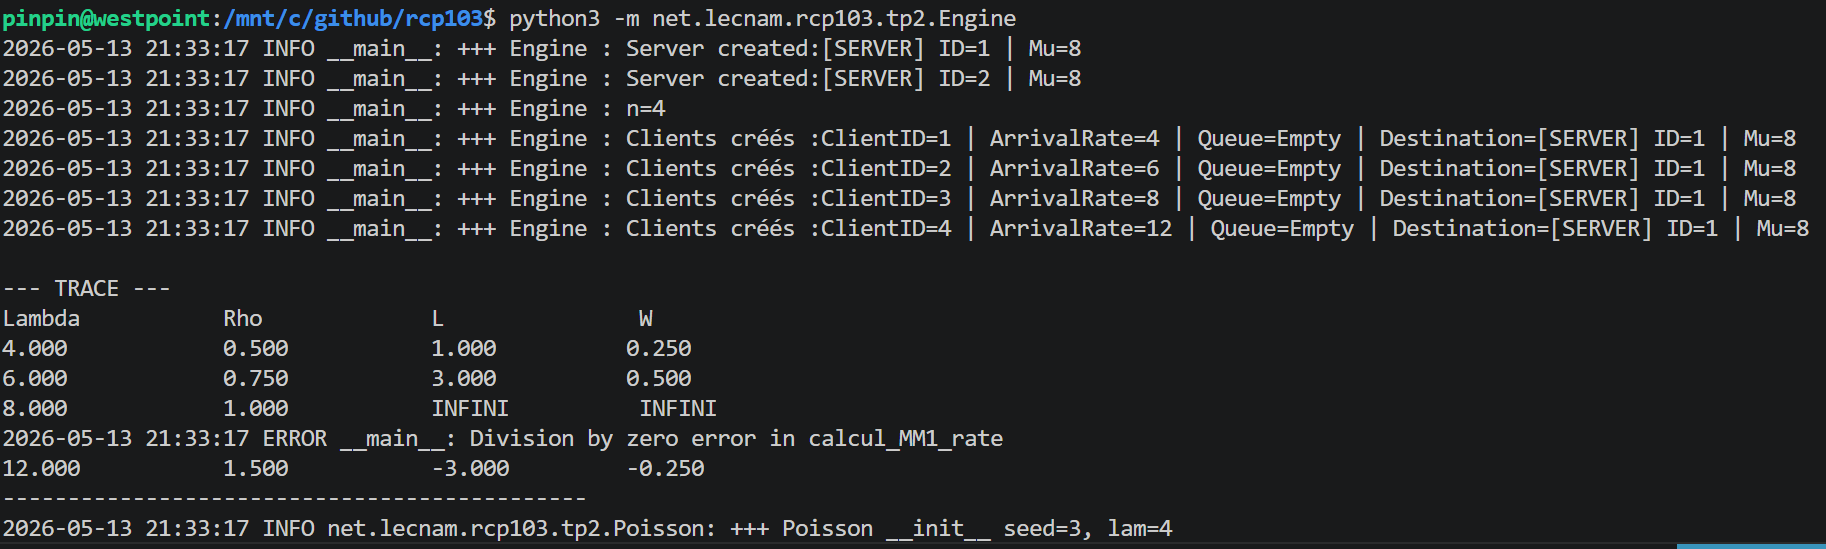
\includegraphics[width=1\linewidth]{capture_logs_seance2_1.png}
    \caption{Affichage du tableau théorique M/M/1 avec les valeurs de \(\lambda\), \(\rho\), \(L\) et \(W\)}
    \label{fig:logs-seance2-1}
\end{figure}

La figure~\ref{fig:logs-seance2-1} constitue la validation principale. Elle montre que le programme affiche bien le tableau des valeurs théoriques de la file M/M/1. On vérifie notamment la présence de la ligne correspondant à \(\lambda = 8\), pour laquelle les colonnes \(L\) et \(W\) affichent \texttt{INFINI}. Cet affichage confirme que le cas de division par zéro est bien pris en compte dans le code.

\begin{figure}[H]
    \centering
    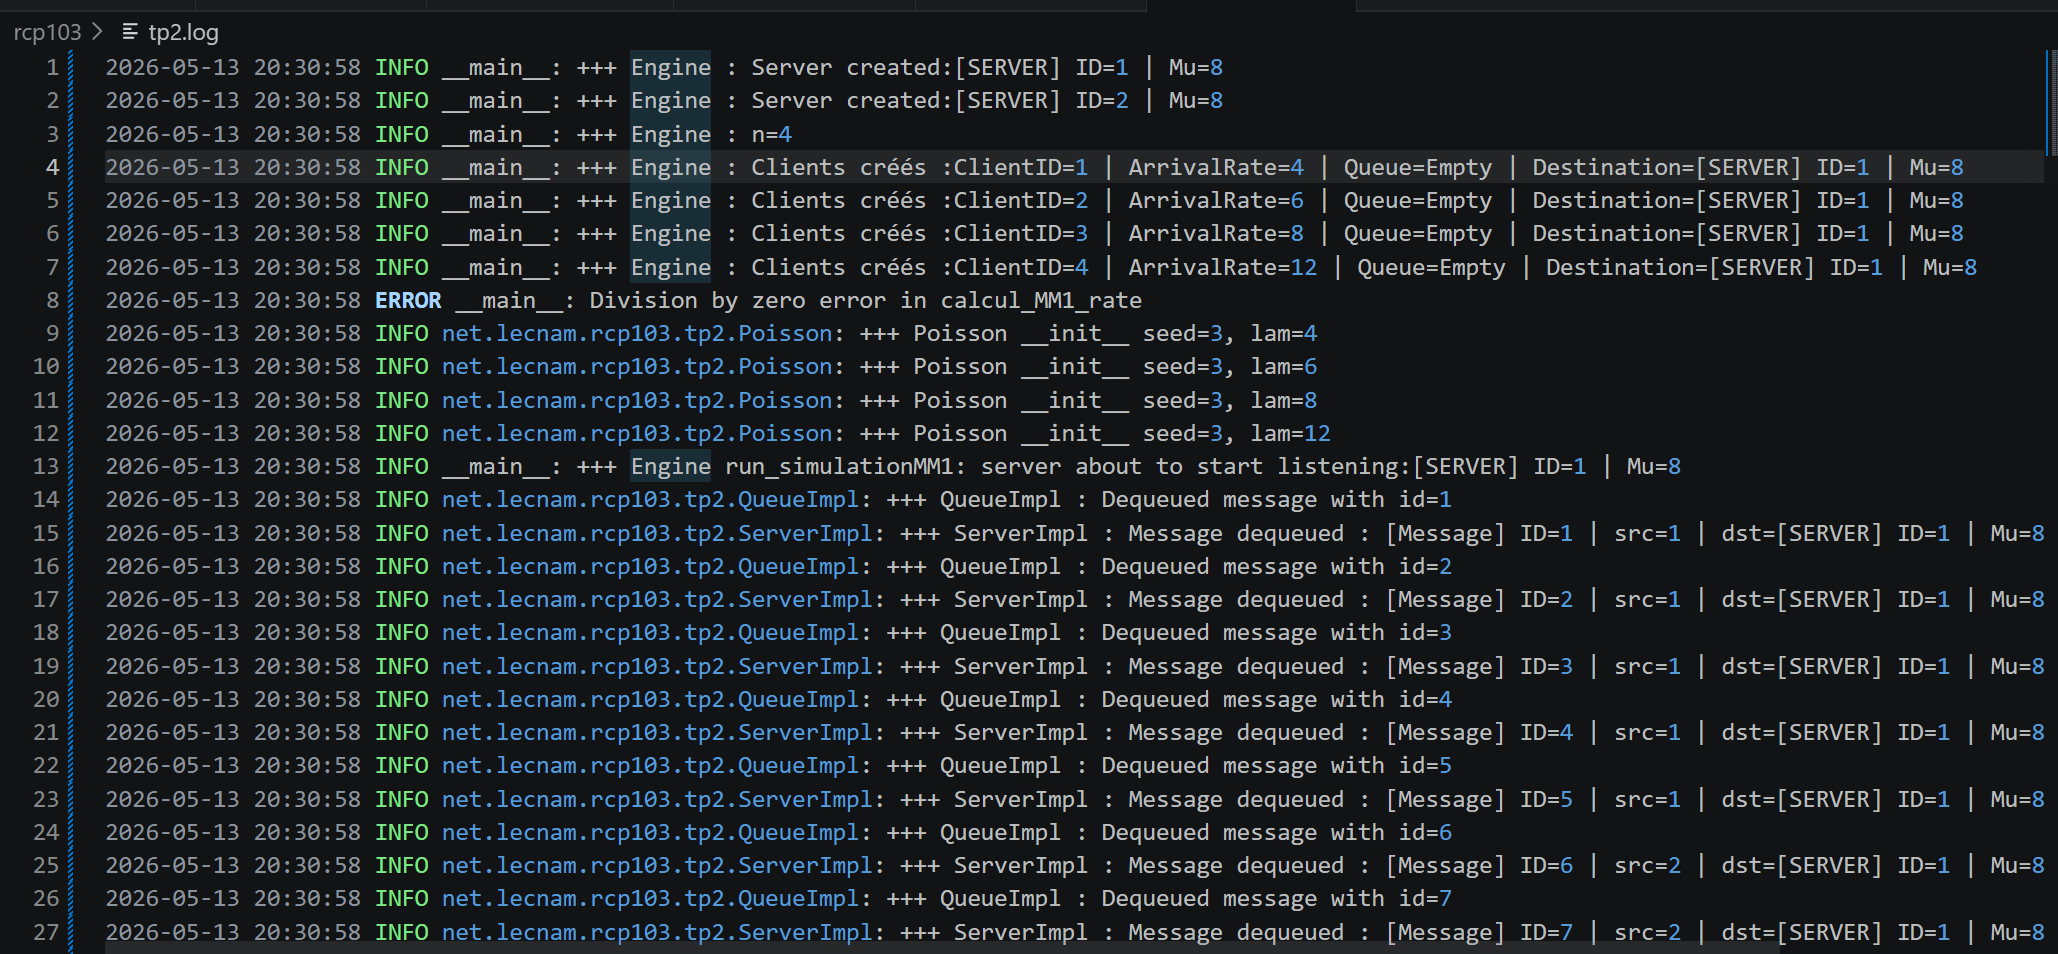
\includegraphics[width=1\linewidth]{capture_logs_seance2_2.png}
    \caption{Première capture d'écran des logs de la séance 2}
    \label{fig:logs-seance2-2}
\end{figure}

\begin{figure}[H]
    \centering
    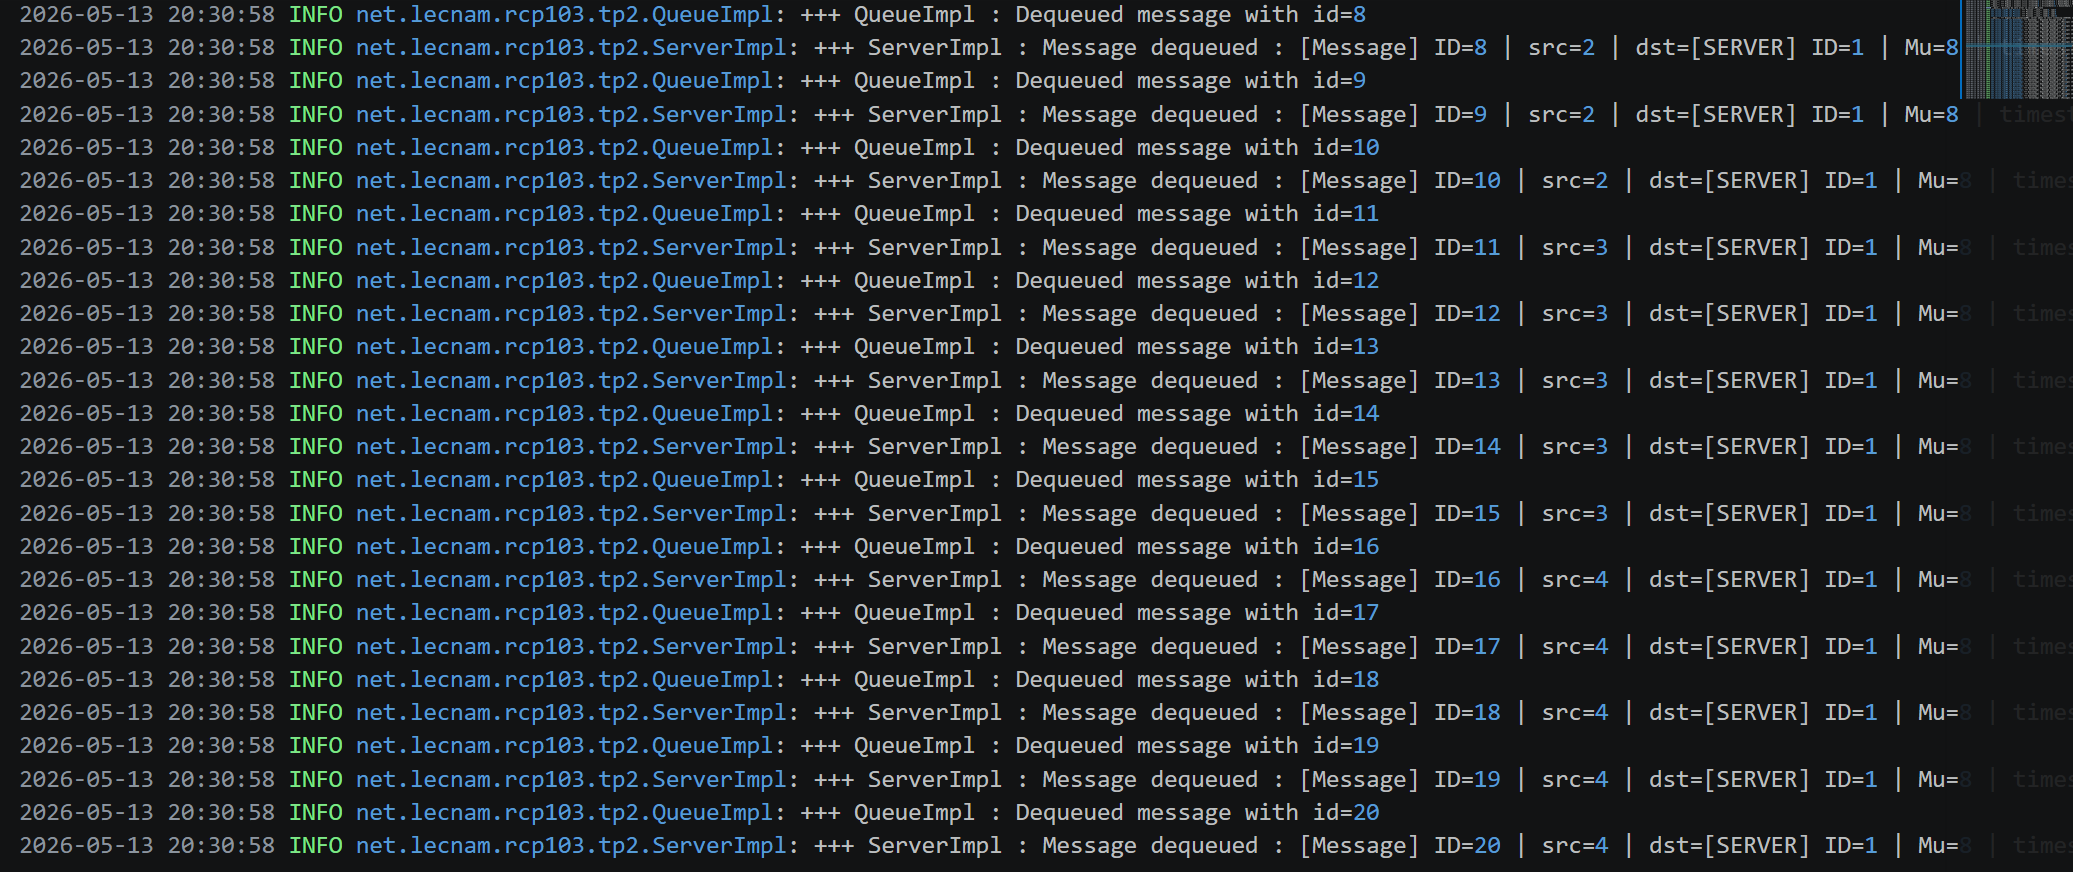
\includegraphics[width=1\linewidth]{capture_logs_seance2_3.png}
    \caption{Fin d'exécution et traces de fermeture de la méthode \texttt{calcul\_MM1\_rate}}
    \label{fig:logs-seance2-3}
\end{figure}

\subsection{Apport de cette validation}

Ces captures d'écran complètent les tests unitaires et les extraits de code présentés précédemment. Elles prouvent que :
\begin{itemize}[leftmargin=*]
    \item le moteur \texttt{Engine.py} est bien exécuté ;
    \item la méthode \texttt{calcul\_MM1\_rate} est appelée ;
    \item les valeurs théoriques M/M/1 sont calculées ;
    \item le cas limite \(\lambda = \mu\) est correctement détecté ;
    \item l'affichage \texttt{INFINI} est bien produit ;
    \item les logs permettent de suivre le début et la fin de l'exécution.
\end{itemize}

Cette validation donne donc une preuve concrète du bon fonctionnement du code pour la partie théorique M/M/1 demandée dans le TP.

\section{Intégration avec le scheduler}

\subsection{Rappel du rôle du scheduler}

Le scheduler reste responsable de l’organisation temporelle des événements. Il stocke les événements futurs et les restitue dans l’ordre chronologique.

Son interface minimale contient notamment :

\begin{lstlisting}[language=Python, caption=Extrait de IScheduler.py]
class IScheduler(ABC):

    @abstractmethod
    def add_event(self, event: IEvent):
        pass
\end{lstlisting}

\subsection{Lien avec les nouveaux composants}

Les composants introduits en séance 2 interagiront avec le scheduler de la manière suivante :
\begin{itemize}[leftmargin=*]
    \item le client génère des événements \texttt{SEND\_MSG} ;
    \item la passerelle génère des événements \texttt{RECV\_MSG} ;
    \item le serveur génère des événements \texttt{MSG\_DEPT} ;
    \item la file d’attente influence la date de début de service d’un message ;
    \item le moteur extrait les événements du scheduler et déclenche les traitements associés.
\end{itemize}

\subsection{Scénario conceptuel}

Un scénario simple peut être décrit ainsi :
\begin{enumerate}[leftmargin=*]
    \item le client crée un message au temps \(t\) ;
    \item un événement \texttt{SEND\_MSG} est ajouté au scheduler ;
    \item lorsque l’événement est traité, un événement \texttt{RECV\_MSG} est programmé à \(t + d\), où \(d\) est le délai de propagation ;
    \item à la réception, si un serveur est libre, le message est traité immédiatement ;
    \item sinon, le message est inséré dans \texttt{QueueImpl} ;
    \item à la fin du service, un événement \texttt{MSG\_DEPT} est traité ;
    \item si la file contient un message, celui-ci est extrait et servi.
\end{enumerate}

\section{Préparation des métriques}

\subsection{Métriques attendues}

Les métriques prévues dans le sujet sont :
\begin{itemize}[leftmargin=*]
    \item le nombre instantané de requêtes dans le système ;
    \item le nombre instantané de requêtes dans la file ;
    \item le nombre total d’arrivées ;
    \item le nombre total de départs ;
    \item le nombre de messages rejetés ;
    \item le nombre moyen de requêtes dans le système ;
    \item le nombre moyen de requêtes dans la file ;
    \item le temps moyen dans le système ;
    \item le temps moyen en file ;
    \item le débit.
\end{itemize}

\subsection{Temps de séjour}

Le timestamp du message permet de calculer le temps total passé dans le système :

\[
W_{\text{système},i} =
t_{\text{départ},i} - t_{\text{création},i}
\]

Le temps moyen dans le système est alors :

\[
\overline{W}_{\text{système}} =
\frac{1}{N}
\sum_{i=1}^{N}
\left(
t_{\text{départ},i} - t_{\text{création},i}
\right)
\]

\subsection{Nombre moyen de messages}

Le nombre moyen de messages dans le système est une moyenne temporelle. Si \(N_i\) est le nombre de messages dans le système pendant l’intervalle \(\Delta t_i\), alors :

\[
\overline{N} =
\frac{1}{T}
\sum_i N_i \Delta t_i
\]

Cette métrique nécessite de mettre à jour l’aire sous la courbe \(N(t)\) à chaque événement.

\subsection{Loi de Little}

La loi de Little fournit une relation de cohérence entre le nombre moyen de messages, le débit et le temps moyen :

\[
L = \lambda W
\]

Dans la séance 3, cette loi pourra être utilisée pour vérifier les résultats expérimentaux du simulateur.

\section{Lien avec les modèles de file d’attente}

\subsection{Modèle M/M/1}

Le modèle M/M/1 correspond à :
\begin{itemize}[leftmargin=*]
    \item une arrivée markovienne ;
    \item un temps de service markovien ;
    \item un serveur unique ;
    \item une file de capacité infinie.
\end{itemize}

Pour ce modèle, les formules théoriques sont :

\[
\rho = \frac{\lambda}{\mu}
\]

\[
L = \frac{\rho}{1-\rho}
\]

\[
W = \frac{1}{\mu-\lambda}
\]

La condition de stabilité est :

\[
\rho < 1
\quad \Longleftrightarrow \quad
\lambda < \mu
\]

\subsection{Modèles M/M/1/K}

Les modèles M/M/1/4 et M/M/1/8 ajoutent une capacité maximale \(K\). Lorsque le système contient déjà \(K\) messages, toute nouvelle arrivée est rejetée.

La file \texttt{QueueImpl} devra donc permettre de détecter l’état plein du système.

\subsection{Modèle M/M/3/8}

Le modèle M/M/3/8 introduit trois serveurs partageant une même file. La classe \texttt{ServerImpl} doit donc pouvoir être instanciée plusieurs fois, et le moteur doit être capable de sélectionner un serveur libre.

La création de plusieurs serveurs dans \texttt{Engine.py} :

\begin{lstlisting}[language=Python]
engine.create_servers(2)
\end{lstlisting}

prépare cette logique multi-serveurs.

\section{Synthèse de la séance 2}

La séance 2 a permis d’ajouter au simulateur les composants opérationnels nécessaires à la modélisation d’une file d’attente. Les principales avancées sont :
\begin{itemize}[leftmargin=*]
    \item l’introduction de la classe \texttt{ClientImpl} pour représenter les générateurs de messages ;
    \item l’introduction de la classe \texttt{QueueImpl} pour représenter la file d’attente ;
    \item l’introduction de la classe \texttt{ServerImpl} pour représenter les serveurs ;
    \item la mise en place de la classe \texttt{ConfigImpl} pour centraliser les paramètres ;
    \item la préparation des distributions aléatoires avec \texttt{Distribution} et \texttt{Poisson} ;
    \item l’évolution de \texttt{Engine.py} vers un rôle d’orchestrateur ;
    \item l’ajout de tests séparés pour les nouveaux composants ;
    \item la préparation des métriques qui seront exploitées lors de la séance 3.
\end{itemize}

Ces éléments complètent les fondations posées lors de la première séance. Le simulateur dispose maintenant des objets nécessaires pour représenter les entités principales d’un système client--file--serveur.

\section{Conclusion}

Cette deuxième séance constitue une étape intermédiaire importante dans la construction du simulateur à événements discrets. Après la mise en place des messages, événements et du scheduler lors de la séance 1, le projet introduit maintenant les composants qui décrivent le comportement opérationnel du système : clients, file d’attente et serveurs.

La classe \texttt{ClientImpl} prépare la génération de messages et d’événements d’arrivée. La classe \texttt{QueueImpl} permet de représenter les messages en attente selon une logique FIFO. La classe \texttt{ServerImpl} prépare la modélisation du traitement et des événements de départ. La classe \texttt{ConfigImpl} centralise les paramètres et le logging, tandis que les classes \texttt{Distribution} et \texttt{Poisson} préparent la génération aléatoire nécessaire aux modèles probabilistes.

Le moteur \texttt{Engine.py} commence à intégrer ces composants en créant plusieurs clients et plusieurs serveurs. Cette évolution prépare directement la séance 3, qui consistera à assembler le simulateur complet, à implémenter la passerelle, à générer les traces finales et à comparer les résultats expérimentaux aux formules théoriques des modèles M/M/1, M/M/1/K et M/M/c/K.

\newpage
\appendix

\section{Annexe A -- \texttt{ConfigImpl.py}}

\begin{lstlisting}[language=Python, caption=ConfigImpl.py]
# !/usr/bin/python3

#####################################################################
#
# PYTHONPATH=. /usr/bin/python3 net/lecnam/rcp103/tp2/ConfigImpl.py
#
# #####################################################################

import os
import logging
import logging.config

from net.lecnam.rcp103.SimulateurException import SimulateurException
from net.lecnam.rcp103.tp2.IConfig import IConfig

# Always load logging_config.py from the same directory as this file
config_path = os.path.join(os.path.dirname(__file__), "logging_config.cnf")
logging.config.fileConfig(config_path, defaults=None, disable_existing_loggers=False, encoding=None)

logger = logging.getLogger(__name__)
# https://docs.python.org/3/library/logging.html#logging-levels

# Class d'Implémentation
class ConfigImpl(IConfig):

    SEED= 3 # correspond au Groupe 3
    OUPUT_DIR = "RCP103_TP2_OUTPUTS"
    LOG_CFG_FILE_PATH = "logging_config.cnf"
    
    def __init__(self):
        logger.debug(f"+++ ConfigImpl : START Constructor")
        logger.debug(f"+++ ConfigImpl : END Constructor")
        pass

    def get_seed(self) -> int:
        return self.SEED
    
    def get_output_dir(self) -> str:
        return self.OUPUT_DIR

    def get_log_cfg_file_path(self) -> str:
        return self.LOG_CFG_FILE_PATH

    # --- Affichage ---
    def print_config(self):
        return(f"[Config] seed={self.SEED} | output_dir={self.OUPUT_DIR} | log_cfg_file_path={self.LOG_CFG_FILE_PATH}")
\end{lstlisting}

\section{Annexe B -- \texttt{ClientImpl.py}}

\begin{lstlisting}[language=Python, caption=ClientImpl.py]
# !/usr/bin/python3

#####################################################################
#
# PYTHONPATH=. /usr/bin/python3 net/lecnam/rcp103/tp2/ClientImpl.py
#
# #####################################################################

from abc import abstractmethod
import datetime
import os
import platform
import queue
import string
import sys
import secrets
import traceback

import logging
import logging.config

# from scipy.stats import poisson
# https://docs.scipy.org/doc/scipy/reference/generated/scipy.stats.poisson.html

import numpy as np
import matplotlib.pyplot as plt

from net.lecnam.rcp103.tp2.IEvent import IEvent
from net.lecnam.rcp103.tp2.IMessage import IMessage
from net.lecnam.rcp103.tp2.EventType import EventType
from net.lecnam.rcp103.tp2.IClient import IClient
from net.lecnam.rcp103.tp2.ConfigImpl import ConfigImpl
from net.lecnam.rcp103.SimulateurException import SimulateurException
from net.lecnam.rcp103.tp2 import IQueue
from net.lecnam.rcp103.tp2.Poisson import Poisson
from net.lecnam.rcp103.tp2.Poisson import Distribution
from net.lecnam.rcp103.tp2.QueueImpl import QueueImpl
from net.lecnam.rcp103.tp2.IServer import IServer

cfg = ConfigImpl()
log_path = cfg.get_log_cfg_file_path()

# Always load logging_config.py from the same directory as this file
config_path = os.path.join(os.path.dirname(__file__), log_path)
logging.config.fileConfig(config_path, defaults=None, disable_existing_loggers=False, encoding=None)

logger = logging.getLogger(__name__)
# https://docs.python.org/3/library/logging.html#logging-levels

# Class d'Implémentation
class ClientImpl(IClient):

    message: IMessage
    arrival_rate: int # arrival rate (lambda) of the Poisson distribution
    queue: IQueue
    client_id: int
    destination: IServer

    def __init__(self, arrival_rate: int, q:IQueue):
        logger.debug(f"+++ ClientImpl : START Constructor")

        seed = cfg.get_seed()
        logger.debug(f"+++ ClientImpl : seed={seed}")
        logger.debug(f"+++ ClientImpl : arrival_rate={arrival_rate}")
        self.arrival_rate = arrival_rate

        self.queue = q
        
        logger.debug(f"+++ ClientImpl : END Constructor")

    def send_message(self, msg: IMessage):
        logger.debug(f"+++ ClientImpl : START send_message")
        self.queue.enqueue(msg)
        logger.debug(f"+++ ClientImpl : END send_message")

    def set_client_id(self, id: int):
        self.client_id = id

    def get_client_id(self):
        return self.client_id
    
    def get_destination(self):
        return self.destination

    def set_destination(self, dst: IServer):
        self.destination = dst

    def get_arrival_rate(self):
        return self.arrival_rate

    def set_arrival_rate(self, rate: int):
        self.arrival_rate = rate

    def set_message(self, msg: IMessage):
        self.message = msg

    def get_message(self, msg: IMessage):
        return self.message

    # --- Affichage ---
    def print_client(self):
        logger.debug(f"+++ ClientImpl : START print_client")
        
        # msg = self.message.print_message()
        if not self.queue.is_empty():
            q = self.queue.print_queue()
        else:
            q = "Empty"

        srv = self.destination.print_server()
        client  = f"ClientID={self.client_id} | ArrivalRate={self.arrival_rate} | Queue={q} | Destination={srv}"     
        logger.debug(f"+++ ClientImpl : Client " + str(client)) 
        logger.debug(f"+++ ClientImpl : END print_client")        
        return(client)
\end{lstlisting}

\section{Annexe C -- \texttt{QueueImpl.py}}

\begin{lstlisting}[language=Python, caption=QueueImpl.py]
# !/usr/bin/python3

#####################################################################
#
# PYTHONPATH=. /usr/bin/python3 net/lecnam/rcp103/tp2/QueueImpl.py
#
# #####################################################################

import datetime
import os
import platform
import string
import sys
import secrets
import traceback

import logging
import logging.config

from net.lecnam.rcp103.tp2.IQueue import IQueue
from net.lecnam.rcp103.tp2.ConfigImpl import ConfigImpl
from net.lecnam.rcp103.SimulateurException import SimulateurException

import queue
import numpy as np

from net.lecnam.rcp103.tp2.IMessage import IMessage

cfg = ConfigImpl()
log_path = cfg.get_log_cfg_file_path()

# Always load logging_config.py from the same directory as this file
config_path = os.path.join(os.path.dirname(__file__), log_path)
logging.config.fileConfig(config_path, defaults=None, disable_existing_loggers=False, encoding=None)

logger = logging.getLogger(__name__)
# https://docs.python.org/3/library/logging.html#logging-levels

# Class d'Implémentation
class QueueImpl(IQueue):
 
    queue_size = -1 # If maxsize is <= 0, the queue size is infinite.
    queue: list[IMessage]
    # mu: int # service rate (mu) of the M/M/1 queue
    # lam: int # arrival rate (lambda) of the Poisson distribution
            
    def __init__(self):
        logger.debug(f"+++ QueueImpl : START Constructor")
        self.queue = []
        logger.debug(f"+++ QueueImpl : END Constructor")

    def enqueue(self, msg: IMessage):
        logger.debug(f"+++ QueueImpl : START enqueue")
        self.queue.append(msg)
        logger.debug(f"+++ QueueImpl : END enqueue")    

    def dequeue(self):
        logger.debug(f"+++ QueueImpl : START dequeue")
        if len(self.queue) == 0:
            logger.error(f"+++ QueueImpl : dequeue called on an empty queue")
            return None
        else:
            msg = self.queue.pop(0) # [1, 2, 3, 4] -> pop(0) -> 1
            logger.info(f"+++ QueueImpl : Dequeued message with id={msg.get_message_id()}")
            logger.debug(f"+++ QueueImpl : END dequeue")
            return msg
        
    def count_messages(self):
        logger.debug(f"+++ QueueImpl : START count_messages")
        nb_msg = len(self.queue)
        logger.debug(f"+++ QueueImpl : count_messages = {nb_msg}")
        logger.debug(f"+++ QueueImpl : END count_messages")
        return nb_msg

    def is_empty(self):
        #logger.debug(f"+++ QueueImpl : START is_empty")
        empty = len(self.queue) == 0
        #logger.debug(f"+++ QueueImpl : is_empty = {empty}")
        #logger.debug(f"+++ QueueImpl : END is_empty")
        return empty

    """ --- Affichage de TOUS les messages --- """
    def print_messages(self):
        logger.debug(f"+++ QueueImpl : START print_messages")

        if not self.is_empty():
            for msg in self.queue:
                all_messages += msg.print_message()
                
            logger.info(all_messages)
            return all_messages
        else:
            logger.info(f"+++ QueueImpl : No messages in the queue to print.")
            return None
        logger.debug(f"+++ QueueImpl : END print_messages")
\end{lstlisting}

\section{Annexe D -- \texttt{ServerImpl.py}}

\begin{lstlisting}[language=Python, caption=ServerImpl.py]
# !/usr/bin/python3

#####################################################################
#
# PYTHONPATH=. /usr/bin/python3 net/lecnam/rcp103/tp2/ServerImpl.py
#
# #####################################################################

import datetime
import os
import platform
import string
import sys
import secrets
import traceback

import logging
import logging.config

from time import time, sleep

import numpy as np

from net.lecnam.rcp103.tp2.IEvent import IEvent
from net.lecnam.rcp103.tp2.IMessage import IMessage
from net.lecnam.rcp103.tp2.EventType import EventType
from net.lecnam.rcp103.tp2.IClient import IClient
from net.lecnam.rcp103.tp2.IQueue import IQueue
from net.lecnam.rcp103.tp2.IServer import IServer
from net.lecnam.rcp103.tp2.ConfigImpl import ConfigImpl
from net.lecnam.rcp103.SimulateurException import SimulateurException

try:
    cfg = ConfigImpl()
    log_path = cfg.get_log_cfg_file_path()

    # Always load logging_config.py from the same directory as this file
    config_path = os.path.join(os.path.dirname(__file__), log_path)
    logging.config.fileConfig(config_path, defaults=None, disable_existing_loggers=False, encoding=None)

    logger = logging.getLogger(__name__)
    # https://docs.python.org/3/library/logging.html#logging-levels

except Exception as e:
    # Fallback to basic logging if config file fails
    logging.basicConfig(level=logging.DEBUG, format='%(asctime)s - %(name)s - %(levelname)s - %(message)s')
    logger = logging.getLogger(__name__)
    logger.error(f"Failed to load logging config from {config_path}: {e}")

# Class d'Implémentation
class ServerImpl(IServer):

    mu: int # service rate (mu) of the M/M/1 queue
    server_id: int

    queue: IQueue
    
    def __init__(self, mu: int, server_id: int, queue: IQueue):
        logger.debug(f"+++ ServerImpl : START Constructor")

        self.mu = mu
        self.server_id = server_id
        self.queue = queue

        logger.debug(f"+++ ServerImpl : END Constructor")
    
    def get_queue(self) -> IQueue:
        return self.queue

    def set_queue(self, queue: IQueue):
        self.queue = queue

    def get_server_id(self):
        return self.server_id

    def set_server_id(self, server_id: int):
        self.server_id = server_id

    def listen(self):
        logger.debug(f"+++ ServerImpl : START listen")

        # Loop on Queue messages to dequeue and process them
        while True:
            if not self.queue.is_empty():
                msg = self.queue.dequeue()
                logger.info(f"+++ ServerImpl : Message dequeued : {msg.print_message()}")
                # Process the message (e.g., simulate service time, send response, etc.)
                # For simplicity, we just print the message here
            else:
                #logger.debug(f"+++ ServerImpl : Queue is empty, waiting for messages...")
                # Optionally, add a sleep here to avoid busy waiting
                sleep(0.1)

        logger.debug(f"+++ ServerImpl : END listen")

        def get_server_id():
            return self.server_id
    
        def set_server_id(self, server_id: int):
            self.server_id = server_id

    # --- Affichage ---
    def print_server(self):
        logger.debug(f"+++ ServerImpl : START listen")
        # q = self.queue.print_messages()
        srv = f"[SERVER] ID={self.server_id} | Mu={self.mu}"  
        logger.debug(f"+++ ServerImpl : END listen")        
        return(srv)
\end{lstlisting}

\section{Annexe E -- \texttt{Distribution.py}}

\begin{lstlisting}[language=Python, caption=Distribution.py]
#!/usr/bin/python3

# PYTHONPATH=. /usr/bin/python3 net/lecnam/rcp103/Distribution.py

import os
import traceback
import logging
import logging.config

import numpy as np

from net.lecnam.rcp103.tp2.ConfigImpl import ConfigImpl

cfg = ConfigImpl()
log_path = cfg.get_log_cfg_file_path()
config_path = os.path.join(os.path.dirname(__file__), log_path)
logging.config.fileConfig(config_path, defaults=None, disable_existing_loggers=False, encoding=None)
seed = cfg.get_seed()
rng = np.random.default_rng(seed=seed)
logger = logging.getLogger(__name__)

# Classe parente pour les différentes distributions
class Distribution:
    """Classe de base représentant une distribution statistique."""

    def __init__(self, name: str, rng):
        logger.debug(f"+++ Distribution __init__ : START")
        self.name = name
        self.rng = rng
        logger.debug(f"+++ Distribution __init__ : END")

    def generate(self, n: int) -> np.ndarray:
        raise NotImplementedError("La méthode generate() doit être implémentée dans la sous-classe.")

    def __repr__(self):
        return f"{self.__class__.__name__}(name={self.name!r})"

\end{lstlisting}

\section{Annexe F -- \texttt{Poisson.py}}

\begin{lstlisting}[language=Python, caption=Poisson.py]
#!/usr/bin/python3

# PYTHONPATH=. /usr/bin/python3 net/lecnam/rcp103/Poisson.py

import os
import traceback
import logging
import logging.config

import numpy as np

from net.lecnam.rcp103.tp2.ConfigImpl import ConfigImpl
from net.lecnam.rcp103.tp2.Distribution import Distribution

cfg = ConfigImpl()
log_path = cfg.get_log_cfg_file_path()
config_path = os.path.join(os.path.dirname(__file__), log_path)
logging.config.fileConfig(config_path, defaults=None, disable_existing_loggers=False, encoding=None)
logger = logging.getLogger(__name__)

class Poisson(Distribution):
    """Distribution de Poisson."""

    seed = cfg.get_seed()
    rng = np.random.default_rng(seed=seed)

    def __init__(self, rng, lam: float):
        logger.debug(f"+++ Poisson __init__ : START")
        logger.info(f"+++ Poisson __init__ seed={self.seed}, lam={lam}")
        super().__init__(f"Poisson (λ={lam})", rng)
        self.lam = lam
        logger.debug(f"+++ Poisson __init__ : END")

    def generate(self, n: int) -> np.ndarray:
        return self.rng.poisson(self.lam, size=n)
\end{lstlisting}

\section{Annexe G -- Extrait de \texttt{Engine.py}}

\begin{lstlisting}[language=Python, caption=Engine.py]
#!/usr/bin/python3

# Commande pour lancer le programme : 
# PYTHONPATH=. python3 net/lecnam/rcp103/tp2/Engine.py
# en Linux/WSL: python3 -m net.lecnam.rcp103.tp2.Engine
# sous Windows/PowerShell: python Engine.py

from net.lecnam.rcp103.tp2.MessageImpl import MessageImpl
from net.lecnam.rcp103.tp2.EventImpl import EventImpl
from net.lecnam.rcp103.tp2.SchedulerImpl import SchedulerImpl
from net.lecnam.rcp103.tp2.IScheduler import IScheduler
from net.lecnam.rcp103.tp2.IServer import IServer
from net.lecnam.rcp103.tp2.IClient import IClient
from net.lecnam.rcp103.tp2.IQueue import IQueue
from net.lecnam.rcp103.tp2.ServerImpl import ServerImpl
from net.lecnam.rcp103.tp2.ClientImpl import ClientImpl
from net.lecnam.rcp103.tp2.QueueImpl import QueueImpl
from net.lecnam.rcp103.tp2.Poisson import Poisson
from net.lecnam.rcp103.tp2.Poisson import Distribution
from net.lecnam.rcp103.tp2.ConfigImpl import ConfigImpl

import numpy as np

import logging
import logging.config
import os
import platform
import string
import sys

# Always load logging_config.py from the same directory as this file
config_path = os.path.join(os.path.dirname(__file__), "logging_config.cnf")
logging.config.fileConfig(config_path, defaults=None, disable_existing_loggers=False, encoding=None)

logger = logging.getLogger(__name__)
# https://docs.python.org/3/library/logging.html#logging-levels

class Engine:

    nb_clients: int
    nb_servers: int
    lambda_arrival_rate: list
    service_rate: int
    simulation_time: float
    clients: list
    servers: list[IServer]
    scheduler: IScheduler
    queue: IQueue

    def __init__(self):
        logger.debug("+++ Engine : START __init__ ...")
        self.scheduler = SchedulerImpl()
        self.nb_clients = 0
        self.nb_servers = 0
        self.service_rate = 8
        self.lambda_arrival_rate = [4, 6, 8 , 12] # arrival rate (lambda) of the Poisson distribution
        self.simulation_time = 10.0
        self.clients = []
        self.servers = []
        self.queue = QueueImpl()

        logger.debug("+++ Engine : START __init__ ...")

    def create_clients(self, n):
        logger.debug("+++ Engine : START create_clients ...")
        self.nb_clients = n
        self.clients = []

        logger.info(f"+++ Engine : n=" + str(n))
        i=0
        for i in range(1, n + 1):
            logger.debug(f"+++ Engine : i=" + str(i))
            client = ClientImpl(arrival_rate=self.lambda_arrival_rate[i-1], q=self.queue)
            client.set_client_id(i)
            client.set_destination(self.servers[0])
            self.clients.append(client)
            pretty_client = client.print_client()
            logger.info("+++ Engine : Clients créés :" + str(pretty_client))
            i+=1

        logger.debug("+++ Engine : END create_clients ...")
        
    def create_servers(self, n):
        logger.debug("+++ Engine : START create_servers ...")
        self.nb_servers = n
        logger.debug("+++ Engine : START about to create n servers, n=" + str(n))
        self.servers = []
        for i in range(1, n + 1):
            srv = ServerImpl(server_id=i, mu=self.service_rate, queue=self.queue)
            self.servers.append(srv)
            pretty_srv = srv.print_server()
            logger.info("+++ Engine : Server created:" + str(pretty_srv))

        logger.debug("+++ Engine : END create_servers ...")

    def print_trace_header(self):
        print("\n--- TRACE ---")
        print(f"{'time':<8} {'node':<5} {'event':<6} {'src':<5} {'dst':<5} {'msgID':<5}")
        print("-" * 45)

    def generate_trace(self, event):
        msg = event.get_message()

        event_type = event.get_event_type()

        if event_type == "SEND_MSG":
            node = msg.get_source()
            event_name = "SEND"
        elif event_type == "RECV_MSG":
            node = 0
            event_name = "RECV"
        elif event_type == "MSG_DEPT":
            node = 0
            event_name = "DEPT"
        else:
            node = 0
            event_name = event_type

        print(
            f"{event.get_event_time():<8.3f} "
            f"{node:<5} "
            f"{event_name:<6} "
            f"{msg.get_source():<5} "
            f"{msg.get_destination():<5} "
            f"{msg.get_message_id():<5}"
        )

    def run(self):
        self.print_trace_header()

        while self.scheduler.has_events():
            event = self.scheduler.get_event()
            self.generate_trace(event)

    def test_message(self):
        print("\n--- TEST MESSAGE ---")
        msg = MessageImpl(1, 1, 0, 0.0)
        msg.print_message()

    def test_event(self):
        print("\n--- TEST EVENT ---")
        msg = MessageImpl(1, 1, 0, 0.0)
        event = EventImpl(1, msg, "SEND_MSG", 1.567)
        prettyEvt = event.print_event()
        print("+++ Pretty print = " + str(prettyEvt))

    def test_scheduler(self):
        print("\n--- TEST SCHEDULER ---")

        msg1 = MessageImpl(1, 1, 0, 0.0)
        msg2 = MessageImpl(2, 3, 0, 0.0)

        e1 = EventImpl(1, msg1, "SEND_MSG", 1.202)
        e2 = EventImpl(2, msg1, "RECV_MSG", 1.916)
        e3 = EventImpl(3, msg2, "SEND_MSG", 2.320)
        e4 = EventImpl(4, msg2, "RECV_MSG", 2.391)
        e5 = EventImpl(5, msg1, "MSG_DEPT", 4.572)
        e6 = EventImpl(6, msg2, "MSG_DEPT", 5.916)

        self.scheduler.add_event(e5)
        self.scheduler.add_event(e1)
        self.scheduler.add_event(e3)
        self.scheduler.add_event(e6)
        self.scheduler.add_event(e2)
        self.scheduler.add_event(e4)

        self.scheduler.print_scheduler()
        logger.debug("+++ Engine : print_scheduler ...")
        logger.info(self.scheduler.print_scheduler())        

    def run_tests(self):
        logger.debug("+++ Engine : START run_tests ...")
        # self.test_message()
        # self.test_event()
        # self.test_scheduler()
        self.run_simulationMM1()
        
        print("\n--- RUN SIMULATION ---")
        #self.run()
        logger.debug("+++ Engine : END run_tests ...")

    def run_simulationMM1(self):
        logger.debug("+++ Engine : START run_simulationMM1 ...")

        # Iterate on servers and trigget listen() method to process messages in the queue
        for server in self.servers:
            pretty_srv = server.print_server()
            logger.info("+++ Engine run_simulationMM1: server about to start listening:" + str(pretty_srv))            
            server.listen()

        logger.debug("+++ Engine : END run_simulationMM1 ...")

    def calcul_MM1_rate(self):
        logger.debug("+++ Engine : START calcul_MM1_rate ...")
        print("\n--- TRACE ---")
        print(f"{'Lambda'} \t \t {'Rho'} \t \t {'L'} \t \t {'W'}")

        # Iterate lambda_arrival_rate and calculate L, W, rho for each lambda and print the results 
        for lam in self.lambda_arrival_rate:
            rho = lam / self.service_rate
            try:
                # self.lambda_arrival_rate = [4, 6, 8 , 12] 
                L = rho / (1 - rho)
                W = 1 / (self.service_rate - lam)
                print(f"{lam:<8.3f} \t {rho:<8.3f} \t {L:<8.3f} \t{W:<8.3f}")
            except ZeroDivisionError as e:
                print(f"{lam:<8.3f} \t {rho:<8.3f} \t {"INFINI"} \t {"INFINI"}")
                logger.error("Division by zero error in calcul_MM1_rate")
        print("-" * 45)
        logger.debug("+++ Engine : END calcul_MM1_rate ...")

if __name__ == "__main__":
    logger.debug("+++ Engine : Main START ...")
    engine = Engine()
    engine.create_servers(2)
    engine.create_clients(4)

    cfg = ConfigImpl()
    seed = cfg.get_seed()
    rng = np.random.default_rng(seed=seed)
    
    engine.calcul_MM1_rate()

    # Loop on each client to send a message to the server
    i=1
    ts = 0.0
    for client in engine.clients:
        fish = Poisson(rng=rng, lam=client.get_arrival_rate())
        for _ in range(5):
            logger.debug("+++ Engine : i=" + str(i))
            msg = MessageImpl(i, client.get_client_id(), client.get_destination(), ts+0.10)
            message = msg.print_message()
            logger.debug("+++ Engine : message = " , {message})
            inter_arrival_time = fish.generate(1)[0] / 1000.0 # Convert ms to seconds
            ts += inter_arrival_time
            msg.set_timestamp(ts)
            client.send_message(msg)
            i+=1

    engine.run_tests()
    logger.debug("+++ Engine : Main END ...")
\end{lstlisting}

\section{Annexe H -- \texttt{ClientImplTest.py}}

\begin{lstlisting}[language=Python, caption=ClientImplTest.py]
#!/usr/bin/python3

# Commande pour lancer le programme : 
# PYTHONPATH=. python3 net/lecnam/rcp103/tp2/ClientImplTest.py
# en Linux/WSL: python3 -m net.lecnam.rcp103.tp2.ClientImplTest
# sous Windows/PowerShell: python ClientImplTest.py

from datetime import datetime
import traceback
import logging
import os

from net.lecnam.rcp103.tp2.ConfigImpl import ConfigImpl
from net.lecnam.rcp103.tp2.ClientImpl import ClientImpl
from net.lecnam.rcp103.tp2.ServerImpl import ServerImpl
from net.lecnam.rcp103.tp2.QueueImpl import QueueImpl

try:
    cfg = ConfigImpl()
    log_path = cfg.get_log_cfg_file_path()

    # Always load logging_config.py from the same directory as this file
    config_path = os.path.join(os.path.dirname(__file__), log_path)
    logging.config.fileConfig(config_path, defaults=None, disable_existing_loggers=False, encoding=None)

    logger = logging.getLogger(__name__)
    # https://docs.python.org/3/library/logging.html#logging-levels

    logger.debug(f"+++ ClientImplTest : START")
    impl = ClientImpl(6)
    queue = QueueImpl()
    srv = ServerImpl(server_id=21, mu=8, queue=queue)
    
    impl.set_client_id(42)
    impl.set_destination(srv)    
    pretty_print = impl.print_client()

    logger.info(f"+++ ClientImplTest : client = {pretty_print}")

    logger.debug(f"+++ ClientImplTest : END")

except RuntimeError as error:
    logger.error("Erreur au Runtime dans ClientImplTest")
    print(f"A {type(error).__name__} has occurred.")
    exit(42)
except Exception as exception :
        logger.error(f"Exception dans ClientImplTest/Main")
        print(f"A {type(exception).__name__} has occurred.")
        print("")
        traceback.print_exc()
        print("")
        print(exception)
        exit(42)
\end{lstlisting}

\section{Annexe I -- \texttt{QueueImplTest.py}}

\begin{lstlisting}[language=Python, caption=QueueImplTest.py]
#!/usr/bin/python3

# Commande pour lancer le programme : 
# PYTHONPATH=. python3 net/lecnam/rcp103/tp2/QueueImplTest.py
# en Linux/WSL: python3 -m net.lecnam.rcp103.tp2.QueueImplTest
# sous Windows/PowerShell: python QueueImplTest.py

from datetime import datetime
import secrets
import traceback
import logging
import os

from net.lecnam.rcp103.tp2.ConfigImpl import ConfigImpl
from net.lecnam.rcp103.tp2.QueueImpl import QueueImpl
# from net.lecnam.rcp103.tp2.Poisson import Poisson
from net.lecnam.rcp103.tp2 import Distribution

import numpy as np


try:
    cfg = ConfigImpl()
    log_path = cfg.get_log_cfg_file_path()

    # Always load logging_config.py from the same directory as this file
    config_path = os.path.join(os.path.dirname(__file__), log_path)
    logging.config.fileConfig(config_path, defaults=None, disable_existing_loggers=False, encoding=None)

    logger = logging.getLogger(__name__)
    # https://docs.python.org/3/library/logging.html#logging-levels

    logger.debug(f"+++ QueueImplTest : START")

    seed = cfg.get_seed()
    rng = np.random.default_rng(seed=seed)

    #fish = Poisson(rng=secrets.SystemRandom(), lam=4)
    impl = QueueImpl()
    q = impl.print_messages()

    logger.info(f"+++ QueueImplTest : q = {q}")

    logger.debug(f"+++ QueueImplTest : END")

except RuntimeError as error:
    logger.error("Erreur au Runtime dans QueueImplTest")
    print(f"A {type(error).__name__} has occurred.")
    exit(42)
except Exception as exception :
        logger.error(f"Exception dans QueueImplTest/Main")
        print(f"A {type(exception).__name__} has occurred.")
        print("")
        traceback.print_exc()
        print("")
        print(exception)
        exit(42)

\end{lstlisting}

\section{Annexe J -- \texttt{ServerImplTest.py}}

\begin{lstlisting}[language=Python, caption=ServerImplTest.py]
#!/usr/bin/python3

# Commande pour lancer le programme : 
# PYTHONPATH=. python3 net/lecnam/rcp103/tp2/ServerImplTest.py
# en Linux/WSL: python3 -m net.lecnam.rcp103.tp2.ServerImplTest
# sous Windows/PowerShell: python ServerImplTest.py

from datetime import datetime

import traceback
import logging
import os

from net.lecnam.rcp103.tp2.ConfigImpl import ConfigImpl
from net.lecnam.rcp103.tp2.ServerImpl import ServerImpl

from net.lecnam.rcp103.tp2.MessageImpl import MessageImpl
from net.lecnam.rcp103.tp2.IServer import IServer
from net.lecnam.rcp103.tp2.IQueue import IQueue
from net.lecnam.rcp103.tp2.ServerImpl import ServerImpl
from net.lecnam.rcp103.tp2.QueueImpl import QueueImpl
from net.lecnam.rcp103.tp2.Poisson import Poisson
from net.lecnam.rcp103.tp2.Poisson import Distribution

try:
    cfg = ConfigImpl()
    log_path = cfg.get_log_cfg_file_path()

    # Always load logging_config.py from the same directory as this file
    config_path = os.path.join(os.path.dirname(__file__), log_path)
    logging.config.fileConfig(config_path, defaults=None, disable_existing_loggers=False, encoding=None)

    logger = logging.getLogger(__name__)
    # https://docs.python.org/3/library/logging.html#logging-levels

    logger.debug(f"+++ ServerImplTest : START")
    queue = QueueImpl()
    impl = ServerImpl(8, 1, queue)

    pretty_srv = impl.print_server()
    logger.debug("+++ ServerImplTest : Server created:" + str(pretty_srv))

    impl.listen()

    logger.debug(f"+++ ServerImplTest : END")

except RuntimeError as error:
    logger.error(f"Erreur au Runtime dans ServerImplTest")
    print(f"A {type(error).__name__} has occurred.")
    exit(42)
except Exception as exception :
        logger.error(f"Exception dans ServerImplTest/Main")
        print(f"A {type(exception).__name__} has occurred.")
        print("")
        traceback.print_exc()
        print("")
        print(exception)
        exit(42)

\end{lstlisting}

\section{Annexe K -- \texttt{ConfigImplTest.py}}
\begin{lstlisting}[language=Python, caption=ConfigImplTest.py]
#!/usr/bin/python3

# Commande pour lancer le programme : 
# PYTHONPATH=. python3 net/lecnam/rcp103/tp2/ConfigImplTest.py
# en Linux/WSL: python3 -m net.lecnam.rcp103.tp2.ConfigImplTest
# sous Windows/PowerShell: python ConfigImplTest.py

from datetime import datetime
import traceback
import logging
import os

from net.lecnam.rcp103.tp2.ConfigImpl import ConfigImpl

# Always load logging_config.py from the same directory as this file
config_path = os.path.join(os.path.dirname(__file__), "logging_config.cnf")
logging.config.fileConfig(config_path, defaults=None, disable_existing_loggers=False, encoding=None)

logger = logging.getLogger(__name__)
# https://docs.python.org/3/library/logging.html#logging-levels

try:
    logger.debug(f"+++ ConfigImplTest : START")
    cfg = ConfigImpl()
    out_dir = cfg.get_output_dir()
    seed = cfg.get_seed()
    log_path = cfg.get_log_cfg_file_path()
    conf = cfg.print_config()
    logger.info(f"+++ ConfigImplTest : seed= {seed}")
    logger.info(f"+++ ConfigImplTest : out_dir= {out_dir}")
    logger.info(f"+++ ConfigImplTest : log_cfg_file_path= {log_path}")
    logger.info(f"+++ ConfigImplTest : Config created: {conf}")
    logger.debug(f"+++ ConfigImplTest : END")

except RuntimeError as error:
    logger.error("Erreur au Runtime dans ConfigImplTest")
    print(f"A {type(error).__name__} has occurred.")
    exit(42)
except Exception as exception :
        logger.error(f"Exception dans ConfigImplTest/Main")
        print(f"A {type(exception).__name__} has occurred.")
        print("")
        traceback.print_exc()
        print("")
        print(exception)
        exit(42)

\end{lstlisting}

\section{Annexe L -- \texttt{EventImpl.py}}
\begin{lstlisting}[language=Python, caption=EventImpl.py]
# !/usr/bin/python3

# PYTHONPATH=. /usr/bin/python3 net/lecnam/rcp103/tp2/EventImpl.py

# rapport à rédiger: overleaf.com

#####################################################################
#
# pre-req: in VSCode install extension 'Microsoft Python Environments Extension' ('Python Environment Manager' is deprecated)
# https://scipy.org/install/: sudo apt-get install python3-scipy
# test in shell with : pip list

# Install on Windows:
# c:\python314\python.exe -m pip install matplotlib

# https://matplotlib.org/stable/install/index.html
# sudo apt upgrade
# sudo apt install python3-matplotlib
# pip install matplotlib
# python3 -m pip install -U pip
# python3 -m pip install -U matplotlib
#  
# To manually trigger a refresh in VSCode:
# Open the Command Palette (Cmd+Shift+P or Ctrl+Shift+P)
# Run Python Environments: Refresh All Environment Managers
#
# #####################################################################

import datetime
import os
import platform
import string
import sys
import secrets
import traceback

import logging
import logging.config

from net.lecnam.rcp103.SimulateurException import SimulateurException

from scipy.stats import poisson
# https://docs.scipy.org/doc/scipy/reference/generated/scipy.stats.poisson.html


import numpy as np


import matplotlib.pyplot as plt

import scipy

from net.lecnam.rcp103.tp2.IEvent import IEvent
from net.lecnam.rcp103.tp2.IMessage import IMessage
from net.lecnam.rcp103.tp2.EventType import EventType

# print(scipy.__version__) 

# Always load logging_config.py from the same directory as this file
config_path = os.path.join(os.path.dirname(__file__), "logging_config.cnf")
logging.config.fileConfig(config_path, defaults=None, disable_existing_loggers=False, encoding=None)

logger = logging.getLogger(__name__)
# https://docs.python.org/3/library/logging.html#logging-levels

# Class d'Implémentation
class EventImpl(IEvent):

    seed= 3 # correspond au Groupe 3
    OUPUT_DIR = "RCP103_TP2_OUTPUTS"

    eventID: int
    message: IMessage
    eventType: string # EventType – SEND_MSG, RECV_MSG, MSG_DEPT
    eventTime: float # horodatage de l'événement
    
    def __init__(self, eventID: int, message: IMessage, eventType: string, eventTime: float):
        self.eventID = eventID
        self.message = message
        self.eventTime = eventTime

        if eventType not in [e.name for e in EventType]:
            logger.error(f"+++ EventImpl __init__  Invalid event type in Constructor: {eventType}. Must be one of: {[e.name for e in EventType]}")
            raise ValueError(f"Invalid event type. Must be one of: {[e.name for e in EventType]}")
        self.eventType = eventType

    def get_event_time(self) ->  datetime.datetime:
        return self.eventTime

    def get_event_type(self) ->  string:
        return self.eventType

    def set_event_time(self, time: datetime):
        self.eventTime = time

    def set_event_type(self, type: string):

        try:
            logger.debug("+++ EventImpl : START setEventType ...")
            if type not in [e.name for e in EventType]:
                logger.error(f"Invalid event type: {type}. Must be one of: {[e.name for e in EventType]}")
                raise ValueError(f"Invalid event type. Must be one of: {[e.name for e in EventType]}")
            self.eventType = type
            logger.debug("+++ EventImpl : evtType = " + str(type))
            logger.debug("+++ EventImpl : END setEventType ...")
        except KeyError:
            raise ValueError(f"Invalid event type: {type}. Must be one of: {[e.name for e in EventType]}")

    def get_message(self) -> IMessage:
        return self.message
    
    def set_message(self, message: IMessage):
        self.message = message
        
    def get_event_id(self) -> int:
        return self.eventID
    
    def set_event_id(self, id: int):
        self.eventID = id

    def print_event(self):
        msg = self.get_message().print_message()
        logger.debug(f"+++ EventImpl : START print_event msg={msg}")
        return(f"Event ID: {self.eventID}, Type: {self.eventType}, Time: {self.eventTime}, Message: {msg}\n")
\end{lstlisting}

\section{Annexe M -- \texttt{EventImplMockTest.py}}
\begin{lstlisting}[language=Python, caption=EventImplMockTest.py]
#!/usr/bin/python3
# PYTHONPATH=. python3 net/lecnam/rcp103/tp2/EventImplMockTest.py
# Use unittest.mock to create a mock SimulateurImpl for Mock testing
# https://docs.python.org/3/library/unittest.mock.html

import traceback
import logging

import unittest
from unittest.mock import MagicMock
from net.lecnam.rcp103.tp2.EventImpl import EventImpl
from net.lecnam.rcp103.tp2.IEvent import IEvent
from net.lecnam.rcp103.tp2.IMessage import IMessage
from net.lecnam.rcp103.tp2.MessageImpl import MessageImpl
from net.lecnam.rcp103.tp2.EventType import EventType

class EventImplMockTest(unittest.TestCase):

    def test_create_class_call_method(self):
        # Create a mock instance of EventImpl
        mock_sim = MagicMock(spec=EventImpl)

        # Example: set return value for calcul
        msg = MessageImpl(1, "Alice", "Bob", 1.64)
        mock_sim.get_message.return_value = msg

        mock_sim.get_event_time.return_value = 1.42
        mock_sim.get_event_type.return_value = "SEND_MSG" # "Fake Foo Event"
        mock_sim.get_event_id.return_value = 42

        # Use the mock in your test
        t = mock_sim.get_event_time()
        type = mock_sim.get_event_type()
        id = mock_sim.get_event_id()

        print("Mocked id:", id)
        print("Mocked type:", type)
        print("Mocked t:", t)

        # You can also assert calls
        mock_sim.get_event_time.assert_called_once()
        self.assertEqual(t, 1.42)
        self.assertEqual(type, "SEND_MSG")
        self.assertEqual(id, 42)

if __name__ == '__main__':
    unittest.main()
\end{lstlisting}

\section{Annexe N -- \texttt{EventImplTest.py}}
\begin{lstlisting}[language=Python, caption=EventImplTest.py]
#!/usr/bin/python3

# Commande pour lancer le programme : 
# PYTHONPATH=. python3 net/lecnam/rcp103/tp2/EventImplTest.py
# en Linux/WSL: python3 -m net.lecnam.rcp103.tp2.EventImplTest
# sous Windows/PowerShell: python EventImplTest.py

from datetime import datetime
import traceback
import logging

from net.lecnam.rcp103.tp2.EventImpl import EventImpl
from net.lecnam.rcp103.tp2.IEvent import IEvent
from net.lecnam.rcp103.tp2.IMessage import IMessage
from net.lecnam.rcp103.tp2.MessageImpl import MessageImpl
from net.lecnam.rcp103.tp2.EventType import EventType

try:
    print("+++ START EventImpl fire")
    msg = MessageImpl(1, "Alice", "Bob", 1.13)
    impl = EventImpl(1, msg, "SEND_MSG", 1.13) # SEND_MSG_ZZZ will force test to fail
    horodatage = impl.get_event_time()
    print("+++ result = " + str(horodatage))
    res = impl.print_event()
    print("+++ pretty print = " + str(res))
    print("+++ END EventImpl ignite")

except RuntimeError as error:
    print("Erreur au Runtime dans EventImpl")
    print(f"A {type(error).__name__} has occurred.")
    exit(42)
except Exception as exception :
        print("Exception dans EventImpl/Main")
        print(f"A {type(exception).__name__} has occurred.")
        print("")
        traceback.print_exc()
        print("")
        print(exception)
        exit(42)
\end{lstlisting}

\section{Annexe O -- \texttt{EventType.py}}
\begin{lstlisting}[language=Python, caption=EventType.py]
from enum import Enum

## EventType – SEND_MSG, RECV_MSG, MSG_DEPT

class EventType(Enum):
    SEND_MSG = 1
    RECV_MSG = 2
    MSG_DEPT = 3
\end{lstlisting}

\section{Annexe P -- \texttt{GatewayImpl.py}}
\begin{lstlisting}[language=Python, caption=GatewayImpl.py]
# !/usr/bin/python3

#####################################################################
#
# PYTHONPATH=. /usr/bin/python3 net/lecnam/rcp103/tp2/GatewayImpl.py
#
# #####################################################################

import datetime
import os
import platform
import string
import sys
import secrets
import traceback

import logging
import logging.config

from net.lecnam.rcp103.tp2.IEvent import IEvent
from net.lecnam.rcp103.tp2.IMessage import IMessage
from net.lecnam.rcp103.tp2.EventType import EventType
from net.lecnam.rcp103.tp2.IClient import IClient
from net.lecnam.rcp103.tp2.IQueue import IQueue
from net.lecnam.rcp103.tp2.IServer import IServer
from rcp103.net.lecnam.rcp103.tp2 import IGateway
from net.lecnam.rcp103.tp2.ConfigImpl import ConfigImpl
from net.lecnam.rcp103.SimulateurException import SimulateurException

cfg = ConfigImpl()
log_path = cfg.get_log_cfg_file_path()

# Always load logging_config.py from the same directory as this file
config_path = os.path.join(os.path.dirname(__file__), log_path)
logging.config.fileConfig(config_path, defaults=None, disable_existing_loggers=False, encoding=None)

logger = logging.getLogger(__name__)
# https://docs.python.org/3/library/logging.html#logging-levels
# Class d'Implémentation
class GatewayImpl(IGateway):

    queue: IQueue
    server: IServer

    def get_queue(self) ->  IQueue:
        return self.queue

    def set_queue(self, queue: IQueue):
        self.queue = queue
    
    def get_server(self) ->  IServer:
        return self.server

    def set_server(self, server: IServer):
        self.server = server

    def __init__(self, queue: IQueue, server: IServer):
        logger.debug(f"+++ GatewayImpl : START Constructor")
        self.queue = queue
        self.server = server
        logger.debug(f"+++ GatewayImpl : END Constructor")

    # --- Affichage ---
    def print_gateway(self):
        logger.debug(f"+++ GatewayImpl : START print_gateway")
        all_msg = self.get_queue().print_messages()
        logger.debug(f"+++ GatewayImpl : Queue messages = {all_msg}")
        srv = self.server.print_server()
        logger.debug(f"+++ GatewayImpl : SERVER = {srv}")
        logger.debug(f"+++ GatewayImpl : END print_gateway")
        return(f"Server: {srv}, ALL Messages: {all_msg}\n")

\end{lstlisting}

\section{Annexe R -- \texttt{IClient.py}}
\begin{lstlisting}[language=Python, caption=IClient.py]

# Interface
from abc import ABC, abstractmethod

from net.lecnam.rcp103.tp2.IMessage import IMessage
from net.lecnam.rcp103.tp2.IServer import IServer


class IClient(ABC):

    @abstractmethod
    def get_destination():
        pass

    # Set Queue name
    @abstractmethod
    def set_destination(dst: IServer):
        pass

    @abstractmethod
    def get_arrival_rate():
        pass

    @abstractmethod
    def set_arrival_rate(rate: int):
        pass

    @abstractmethod
    def send_message(msg: IMessage):
        pass

    @abstractmethod
    def print_client():
        pass

    @abstractmethod
    def set_message(msg: IMessage):
        pass

    @abstractmethod
    def get_message(msg: IMessage):
        pass

    @abstractmethod
    def set_client_id(id: int):
        pass

    @abstractmethod
    def get_client_id():
        pass

    '''
    @abstractmethod
    def foo(x: int, y: int):
        pass
    '''
\end{lstlisting}

\section{Annexe S -- \texttt{IConfig.py}}
\begin{lstlisting}[language=Python, caption=IConfig.py]

# Interface
from abc import ABC, abstractmethod

from net.lecnam.rcp103 import logging_config

class IConfig(ABC):

    @abstractmethod
    def get_seed() -> int:
        pass
    
    def get_output_dir() -> str:
        pass
    
    def get_log_cfg_file_path() -> str:
        pass
    
    # --- Affichage ---
    def print_config():
        pass
\end{lstlisting}

\section{Annexe T -- \texttt{IEvent.py}}
\begin{lstlisting}[language=Python, caption=IEvent.py]
# Interface
from abc import ABC, abstractmethod
import datetime
import string


class IEvent(ABC):

    @abstractmethod
    def get_event_time() ->  datetime.datetime:
        pass

    @abstractmethod
    def get_event_type()  ->  string:
        pass

    @abstractmethod
    def set_event_time(evtString: datetime):
        pass

    @abstractmethod
    def set_event_type(evtType: string):
        pass

    @abstractmethod
    def get_event_id() -> int:
        pass

    @abstractmethod
    def set_event_id(id: int):
        pass

    @abstractmethod
    def print_event():
        pass

    '''
    @abstractmethod
    def foo(x: int, y: int):
        pass
    '''
\end{lstlisting}

\section{Annexe U -- \texttt{IGateway.py}}
\begin{lstlisting}[language=Python, caption=IGateway.py]

# Interface
from abc import ABC, abstractmethod

from net.lecnam.rcp103.tp2 import IGateway
from net.lecnam.rcp103.tp2 import IQueue
from net.lecnam.rcp103.tp2 import IServer

class IGateway(ABC):

    @abstractmethod
    def is_empty(self) -> bool:
        pass

    @abstractmethod
    def get_queue() -> IQueue:
        pass

    @abstractmethod
    def set_queue(q: IQueue):
        pass

    @abstractmethod
    def get_server() -> IServer:
        pass
    
    @abstractmethod
    def set_server(server: IServer):
        pass

    '''
    @abstractmethod
    def foo(x: int, y: int):
        pass
    '''
\end{lstlisting}

\section{Annexe V -- \texttt{IMessage.py}}
\begin{lstlisting}[language=Python, caption=IMessage.py]

# Interface
from abc import ABC, abstractmethod

from net.lecnam.rcp103.tp2.IServer import IServer

class IMessage(ABC):

    @abstractmethod
    def get_source():
        pass

    @abstractmethod
    def get_destination():
        pass

    @abstractmethod
    def get_message_id():
        pass

    @abstractmethod
    def set_source(src: str):
        pass

    @abstractmethod
    def set_destination(dst: IServer):
        pass

    @abstractmethod
    def set_message_id(msg_id: int):
        pass

    @abstractmethod
    def print_message():
        pass

    '''
    @abstractmethod
    def foo(x: int, y: int):
        pass
    '''
\end{lstlisting}

\section{Annexe W -- \texttt{IQueue.py}}
\begin{lstlisting}[language=Python, caption=IQueue.py]

# Interface
from abc import ABC, abstractmethod

from net.lecnam.rcp103.tp2 import IMessage

class IQueue(ABC):

    @abstractmethod
    def is_empty(self) -> bool:
        pass

    @abstractmethod
    def enqueue(msg: IMessage):
        pass

    @abstractmethod
    def dequeue():
        pass

    @abstractmethod
    def count_messages(self):
        pass
    
    @abstractmethod
    def print_messages():
        pass

    '''
    @abstractmethod
    def foo(x: int, y: int):
        pass
    '''
\end{lstlisting}

\section{Annexe X -- \texttt{IScheduler.py}}
\begin{lstlisting}[language=Python, caption=IScheduler.py]

# Interface
from abc import ABC, abstractmethod
import datetime

from .IEvent import IEvent

class IScheduler(ABC):
    @abstractmethod
    def add_event(self, event: IEvent):
        pass

    @abstractmethod
    def get_event(self):
        pass

    @abstractmethod
    def get_current_time(self):
        pass

    @abstractmethod
    def has_events(self):
        pass

    '''
    @abstractmethod
    def foo(x: int, y: int):
        pass
    '''
\end{lstlisting}

\section{Annexe Y -- \texttt{IServer.py}}
\begin{lstlisting}[language=Python, caption=IServer.py]

# Interface
from abc import ABC, abstractmethod

from net.lecnam.rcp103.tp2 import IQueue
from net.lecnam.rcp103.tp2 import IMessage

class IServer(ABC):
        
    @abstractmethod
    def get_queue() -> IQueue:
        pass

    @abstractmethod
    def set_queue(queue: IQueue):
        pass

    @abstractmethod
    def get_server_id():
        pass

    @abstractmethod
    def set_server_id(server_id: int):
        pass

    @abstractmethod 
    def print_server():
        pass
    
    @abstractmethod
    def listen():
        pass

    '''
    @abstractmethod
    def foo(x: int, y: int):
        pass
    '''
\end{lstlisting}

\section{Annexe Z -- \texttt{logging_config.cnf}}
\begin{lstlisting}[language=conf, caption=logging_config.cnf]
[loggers]
keys=root

[handlers]
keys=consoleHandler,fileHandler

[formatters]
keys=simpleFormatter

[logger_root]
level=DEBUG
handlers=consoleHandler,fileHandler

[handler_consoleHandler]
class=StreamHandler
level=DEBUG
formatter=simpleFormatter
args=(sys.stdout,)

[handler_fileHandler]
class=FileHandler
level=DEBUG
formatter=simpleFormatter
args=('tp2.log', 'a')

[formatter_simpleFormatter]
format=%(asctime)s %(levelname)s %(name)s: %(message)s
datefmt=%Y-%m-%d %H:%M:%S
\end{lstlisting}

\section{Annexe AA -- \texttt{Message.py}}
\begin{lstlisting}[language=Python, caption=Message.py]
from .IMessage import IMessage

class Message(IMessage):
    """ Message envoyé vers la passerelle"""

    message_id: int
    source: str
    destination: str
    timestamp: float

    def __init__(self, message_id, source, destination, timestamp=0.0):
        self._message_id = message_id
        self._source = source
        self._destination = destination
        self._timestamp = timestamp 

    ### getters du message ###
    def get_message_id(self):
        return self._message_id

    def get_source(self):
        return self._source

    def get_destination(self):
        return self._destination

    def get_timestamp(self):
        return self._timestamp

    def set_message_id(self, message_id):
        self._message_id = message_id

    def set_source(self, source):
        self._source = source

    def set_destination(self, destination):
        self._destination = destination

    ### setters du message ###
    def set_timestamp(self, temps):
        self._timestamp = temps

    # --- Affichage ---
    def print_message(self):
        message_str = (f"[Message] ID={self._message_id} | src={self._source} "
                       f"| dst={self._destination} | timestamp={self._timestamp:.4f}")
        print(message_str)
        return message_str

\end{lstlisting}

\section{Annexe AB -- \texttt{MessageImpl.py}}
\begin{lstlisting}[language=Python, caption=MessageImpl.py]
from .IMessage import IMessage
from net.lecnam.rcp103.tp2.IServer import IServer

class MessageImpl(IMessage):
    """ Message envoyé vers la passerelle"""

    message_id: int
    source: str
    destination: IServer
    timestamp: float

    def __init__(self, message_id, source, destination, timestamp=0.0):
        self._message_id = message_id
        self._source = source
        self._destination = destination
        self._timestamp = timestamp 

    ### getters du message ###
    def get_message_id(self):
        return self._message_id

    def get_source(self):
        return self._source

    def get_destination(self):
        return self._destination

    def get_timestamp(self):
        return self._timestamp

    def set_message_id(self, message_id):
        self._message_id = message_id

    def set_source(self, source):
        self._source = source

    def set_destination(self, destination):
        self._destination = destination

    ### setters du message ###
    def set_timestamp(self, temps):
        self._timestamp = temps

    # --- Affichage ---
    def print_message(self):
        return(f"[Message] ID={self._message_id} | src={self._source} "
              f"| dst={self._destination.print_server()} | timestamp={self._timestamp:.4f}")
\end{lstlisting}

\section{Annexe AC -- \texttt{MessageImplTest.py}}
\begin{lstlisting}[language=Python, caption=MessageImplTest.py]
#!/usr/bin/python3

# Commande pour lancer le programme : 
# PYTHONPATH=. python3 net/lecnam/rcp103/tp2/MessageImplTest.py
# en Linux/WSL: python3 -m net.lecnam.rcp103.tp2.MessageImplTest
# sous Windows/PowerShell: python MessageImplTest.py

from datetime import datetime
import traceback
import logging

from net.lecnam.rcp103.tp2.EventImpl import EventImpl
from net.lecnam.rcp103.tp2.IEvent import IEvent
from net.lecnam.rcp103.tp2.IMessage import IMessage
from net.lecnam.rcp103.tp2.MessageImpl import MessageImpl

try:
    print("+++ START MessageImplTest fire")
    impl = MessageImpl(1, "Alice", "Bob", 1.21)
    src = impl.get_source()
    dst = impl.get_destination()
    print(f"Source: {src}, Destination: {dst}")
    res = impl.print_message()
    print("+++ Pretty print = " + str(res))   
    print("+++ END MessageImplTest ignite")

except RuntimeError as error:
    print("Erreur au Runtime dans MessageImplTest")
    print(f"A {type(error).__name__} has occurred.")
    exit(42)
except Exception as exception :
        print("Exception dans MessageImplTest/Main")
        print(f"A {type(exception).__name__} has occurred.")
        print("")
        traceback.print_exc()
        print("")
        print(exception)
        exit(42)

\end{lstlisting}

\section{Annexe AD -- \texttt{SchedulerImpl.py}}
\begin{lstlisting}[language=Python, caption=SchedulerImpl.py]
# Interface
from abc import ABC, abstractmethod
import datetime

from net.lecnam.rcp103.tp2.IEvent import IEvent
from net.lecnam.rcp103.tp2.IScheduler import IScheduler

class SchedulerImpl(IScheduler):

    events: list
    current_time: float

    def __init__(self):
        self.events = []
        self.current_time = 0.0

    def add_event(self, event):
        t = event.get_event_time()
        for i, e in enumerate(self.events):
            if (e.get_event_time() > t):
                self.events.insert(i, event)
                return
        self.events.append(event)

    def get_event(self):
        if not self.events:
            return None
        event = self.events.pop(0)
        self.current_time = event.get_event_time()
        return event

    def get_current_time(self):
        return self.current_time

    def has_events(self):
        return bool(self.events)
    
    def print_scheduler(self):
        resultat = ""
        for event in self.events:
            resultat += f"Event ID: {event.eventID}, Type: {event.eventType}, Time: {event.eventTime}\n"
        return resultat
\end{lstlisting}
\end{document}
